%% Quadratic ephemerides over 16-20 yr need not be secular period changes
%% A&A regular article.  Requires aa.cls (and aa.bst if you switch to BibTeX):
%%   https://www.aanda.org/for-authors/latex-issues/texnical-background
%% Figures expected in ./figures/ : fig1_barras.png fig2_v527_injecao.png
%%                                 fig3_cvdra.png  fig4_dpdt.png
%% Compile: pdflatex dpdt_note ; pdflatex dpdt_note
\documentclass{aa}

\usepackage[utf8]{inputenc}
\usepackage[T1]{fontenc}
\usepackage{graphicx}
\usepackage{txfonts}
\usepackage{rotating}
\usepackage[colorlinks,citecolor=blue,urlcolor=blue]{hyperref}
\usepackage{orcidlink}
\hypersetup{pdfauthor={R. Walitte}}

\begin{document}

\title{Quadratic ephemerides over 16--20\,yr need not be secular period changes}
\subtitle{Timing bars and undersampled third-body orbits in 26 short-period eclipsing binaries}

\author{R.~Walitte\orcidlink{0009-0004-1776-2754}\inst{1}}
\authorrunning{Walitte}
\institute{Independent researcher, Rua 05, 76385-286 Goian\'esia, GO, Brazil\\ \email{rondinellewalitte@gmail.com}}

\date{Received ---; accepted ---}

\abstract{Period-change rates of close binaries are measured by fitting a quadratic ephemeris to eclipse timings spanning decades. Underestimated timing errors and unresolved cyclic signals both manufacture a rate in such a fit.}{To measure both effects on a uniformly processed sample and state what a quadratic coefficient over 16--20 yr can mean.}{Eclipse timings of 26 catalogued binaries with P $<$ 5 d from TESS 2-min photometry (2019--2026) and SuperWASP (2004--2008). Timing errors are taken from the data, the SuperWASP bias is calibrated on transiting planets, and every fit carries goodness-of-fit, curvature and adversarial tests. Results are confronted with the VarAstro minima database, with the published third-body orbit of one target, and with the timing of the secondary minima.}{With formal errors the chain returns 24 of 31 targets ``significant'' at 3$\sigma$; with errors from the data, 11 of 26 with curvature surviving an adversarial test. Those bars are still 1.39 times too small (median reduced $\chi^2$ 1.41 against 0.73 expected for 1--4 degrees of freedom). Leverage-corrected residuals locate the excess in the SuperWASP epochs (bars up to 1.65 times too small; injecting the third-body population of Section 6 shows about a fifth of that excess can be undersampled orbits, so the correction is a ceiling and 1.54 the central bar-only value --- and the TESS residuals themselves bound the in-window tertiary fraction to $\lesssim$ 0.5); the TESS epochs are at expectation, but three parameters on four epochs leave the test only 38\% of their variance, so it is nearly blind where the ten detections live. With the SuperWASP bars corrected, 10 of the 11 detections stand; with the TESS bars also inflated to the 95\% limit their residuals allow, 8 stand. Adding to the TESS bars a between-sector drift of the size measured on the secondary minima of five targets --- a ceiling the residuals do not require --- removes all but one: TIC 232634196, carried by the 20-yr lever, surviving the corrected SuperWASP bars, its secondary moving with its primary. Of the eleven, two have an external record long enough to test: one is a published third-body orbit with no secular term (V527 Dra), the other agrees only within our window.}{The archival bars are what the residuals say is wrong --- partly bar, partly the undersampled orbits themselves --- and correcting them to the ceiling leaves the detections in place; what they then rest on is timing structure within five years of TESS, which within-sector bars cannot certify against between-sector noise. Undersampled third-body orbits account for about one of the eight. Quadratic coefficients over 16--20 yr from a few epochs should not be reported as secular rates without bars validated at the between-sector scale and without an external record.}

\keywords{binaries: eclipsing -- stars: fundamental parameters -- methods: data analysis --
          methods: statistical -- techniques: photometric -- ephemerides}

\maketitle

\section{Introduction}\label{s:intro}
Secular period changes in close binaries encode mass transfer, angular-momentum loss and light-travel-time effects, but measuring them requires eclipse timings spanning decades. Population-level measurements with uniform methodology are rare because the archival step is laborious: heterogeneous time systems, unquantified timing biases, and no ground truth internal to the archive. The chain used here was developed on one system (TYC 7024-1046-1 = TIC 142874476), where a SuperWASP epoch from 2006--2008 propagated through a TESS-refined ephemeris sits 22.7 $\pm$ 2.2 min from the linear prediction. This note reports what that chain returns when applied uniformly to every catalogued binary for which the data exist, and --- the part that turned out to matter --- what two external confrontations say about the meaning of the numbers.

\section{Sample selection}\label{s:sel}
Selection is deterministic and every cut is listed with its survivors (Table~\ref{t:funil}). Because a period-change measurement in a population is only interpretable together with its selection function, the targets that were \emph{not} measured are part of the result and are reported with the reason (Table~\ref{t:naomedidos}).
\begin{table}
\caption{Selection funnel.}
\label{t:funil}
\centering
\begin{tabular}{c p{0.62\linewidth} r}
\hline\hline
Step & Criterion & N\\
\hline
1 & Union of the TESS eclipsing-binary catalogues of Prša et al. (2022; 4\,584) and Kostov et al. (2025; 7\,936), de-duplicated by position (5\arcsec) over the merged table & 12\,497\\
2 & Catalogue period P $<$ 5 d & 8\,759\\
3 & $\ge$ 2 TESS 2-min sectors separated by $\ge$ 1 yr among the 22 sector manifests held locally (s19--21, 27--28, 75, 90--105) & 288\\
4 & A SuperWASP source within 20\arcsec (public archive cone search --- the query that lists sources, not the light-curve download; 0 of 288 queries unresolved after retry) & 131\\
5 & $\ge$ 4 independent epoch clusters (TESS sectors + SuperWASP seasons), the minimum for a quadratic ephemeris with $\ge$ 1 degree of freedom & 88\\
6 & Passed all measurement guards (Sect.~\ref{s:met}) & \textbf{26}\\
\hline
\end{tabular}
\end{table}
Two remarks. On step 1: the two catalogues are disjoint by construction (0 TICs in common; 23 positional pairs at 5\arcsec), so the union genuinely adds.
On step 3, a caveat that anyone reproducing the selection needs: \textbf{the sector count is a measure of our cache, not of the sky.} The 22 local manifests cover 21\% of TESS sectors, concentrated in 2019--2020 and 2024--2026, so 288 is a lower bound --- and a \emph{biased} one, because the undercount is not uniform. Querying MAST for eight of the 88 targets showed that the four nearest the northern ecliptic pole have 40--43 sectors of 2-min photometry each, of which the cache held 4; targets at lower ecliptic latitude had 7--13, of which the cache held 3--8. Step 3 therefore penalises targets in the continuous-viewing zones most. The sky distribution of the result follows directly: 21 of the 26 measured targets are in Draco (the others: 2 in Microscopium, 2 in Grus, 1 in Indus), because the cached northern sectors overlap there and SuperWASP covered it in 2004--2008. The sample is a Draco sample with a southern tail, not an all-sky one.
\begin{table*}
\caption{\textbf{The 62 targets of the 88 that were not measured, by the first guard each one failed.} This table is a record of where each target stopped, not a map of what recovery would gain: every target fails at the first guard it meets, and behind the first there is usually another (see the recovery pass below). The ``Nature'' column describes the first reason only.}
\label{t:naomedidos}
\centering
\begin{tabular}{p{0.55\linewidth} c p{0.30\linewidth}}
\hline\hline
Reason & N & Nature\\
\hline
SuperWASP curve with $<$ 500 valid points after cleaning & 21 & archive depth; structural\\
Phase coverage of the eclipse not testable in $\ge$ 1 season block (Sect.~\ref{ss:barras}) & 22 & archive sampling; recoverable with a second archive\\
SuperWASP light-curve download returned an empty file (a different operation from the cone search of Table~\ref{t:funil}, step 4) & 4 & fetch failure without retry in this run; recoverable (retry now implemented)\\
Cycle count between TESS sectors ambiguous (period ladder did not close) & 8 & local sector coverage; intermediate sectors were added from MAST and none was recovered (Appendix~\ref{a:A})\\
No applicable eclipse duration in the catalogue (4 NaN; 1 contact-binary width; 1 W UMa) & 6 & catalogue gap; $T_{14}$ was measured on the TESS curve for five and none was recovered (Appendix~\ref{a:A})\\
Catalogue period error NaN & 1 & catalogue gap\\
\hline
\end{tabular}
\end{table*}
A recovery pass was run on the 8 + 6 ``recoverable'' rows after the main batch (intermediate TESS sectors from MAST for the eight; eclipse durations measured on the TESS curves for the six). It recovered none of them: Table~\ref{t:naomedidos} lists the \emph{first} guard each target failed, and behind the first there was a second in every case. Recovery is therefore not additive across the reasons in Table~\ref{t:naomedidos}, and the count of 26 stands (the per-target outcome is in Appendix~\ref{a:A}).
The 26 measured targets are therefore not a random sample of short-period binaries: they are the subset with deep SuperWASP coverage, eclipses sampled in every season, and unambiguous cycle counts across the TESS sectors held locally.

\section{Method}\label{s:met}

\subsection{Eclipse epochs}\label{ss:epocas}
For each TESS sector we fit a periodic trapezoid of free depth to the PDCSAP light curve (QUALITY = 0, normalised to the 95th percentile) on a fine grid of trial epochs, with the eclipse duration $T_{14}$ from the catalogue and the period from the catalogue, seeded on the catalogue reference epoch so that the primary is fitted rather than the deepest minimum in the curve (in contact systems these differ). The epoch is the $\chi^2$ minimum; the formal error is the $\Delta\chi^2$ = 1 half-width. Sectors are anchored to the most recent one.
For SuperWASP we convert HJD\_UTC to BJD\_TDB (a +1.1 min shift at these dates --- larger than the TESS timing error), fit the same profile per observing season, and require phase coverage of the eclipse in every season ($\ge$ 50 points in eclipse, no empty phase bins in 12). A season whose fitted depth is $\le$ 0 is rejected: the grid has found a $\chi^2$ minimum for a \emph{brightening}, and its ``epoch'' is not that of an eclipse. Five of the first 31 targets had such a season; their between-season dispersion was 82 min against 1.8 min for the rest.

\subsection{Period ladder and cycle count}\label{ss:escada}
Within the TESS sectors the period is refined by a ladder: starting from the two closest sectors, each further sector is added only if its linear residual stays below a tolerance equal to the larger of 3 min and three times the median epoch uncertainty of the target (3 min for 22 of the 26; 4.1--5.5 min for the other four), and the result is discarded if shifting any epoch by $\pm$1 cycle does not worsen $\chi^2$. The ladder returns epochs and residuals in the caller's order (Sect.~\ref{s:val}).
The ladder is \emph{not} used across the 2008--2019 gap: it requires a linear ephemeris, and a real $\mathrm{d}P/\mathrm{d}t$ produces tens of minutes of O$-$C over 19 yr, which the ladder would reject as an unresolved alias. Across the gap the cycle number is the rounded propagation with the TESS-refined period, and the count is accepted only if $\sigma_P$ $\times$ N $<$ 0.25 cycle at the farthest epoch. Any target with $|\mathrm{d}P/\mathrm{d}t|$ $>$ 10 s yr$^{-1}$ is flagged as a suspected cycle-count error rather than a measurement; none of the 26 is.

\subsection{Timing uncertainties from the data}\label{ss:barras}
The formal $\Delta\chi^2$ = 1 error is a photon-noise error. Cycle-to-cycle eclipse-timing scatter from spots and O'Connell-type asymmetries is not in it, and in the SuperWASP data the dispersion between observing seasons exceeds the formal error by a median factor of 3.0 (n = 25 targets of the 26; one record lacks the formal value; interquartile range of the factor 2.1--7.2). We therefore assign each epoch the \emph{larger} of its formal error and the dispersion between independent subsets: the two halves of the sector for TESS, the observing seasons for SuperWASP. Each SuperWASP season enters the fit as its own epoch with this error, added in quadrature to the chain-bias uncertainty of Sect.~\ref{ss:vies}. A target with a single valid season has no red-noise estimate and is not measured. Two limitations of these bars are shown by the data in Sect.~\ref{s:val}: the reduced $\chi^2$ they yield is above what correct bars would give for 1--4 degrees of freedom, and the TESS bar, being a within-sector quantity, cannot contain timing drift between sectors.

\subsection{SuperWASP timing bias}\label{ss:vies}
There is no ground truth internal to the archive, so the timing bias of the SuperWASP chain was calibrated on transiting hot Jupiters --- objects whose clocks do not run --- with TESS ephemerides precise enough to propagate 18 yr. Eclipsing binaries cannot serve as clock calibrators: a first attempt with three gave an astrophysical O$-$C scatter of 31.7 min, against 1.73 min for the hot Jupiters. Of 12 hot Jupiters, 8 yielded epochs and 4 passed the between-season dispersion guard (WASP-18 b, WASP-4 b, WASP-6 b, WASP-19 b); their O$-$C are $-$2.85 $\pm$ 1.07, $-$2.55 $\pm$ 1.52, +0.85 $\pm$ 2.21 and $-$0.64 $\pm$ 2.85 min, consistent with a constant offset ($\chi^2$ = 2.62 for 3 d.o.f.):
chain bias = $-$2.14 $\pm$ 0.78 min.
The bias is subtracted from every SuperWASP epoch and its uncertainty added in quadrature. The four rejected calibrators (between-season bars of 17--951 min) were not discarded silently; the guard that rejected them is the same one applied to every target here.
\textbf{The $\pm$0.78 min is a floor, not an estimate of the bias uncertainty for the eclipsing binaries.} A bias of $-$2.14 min is too large for a time-scale error (the HJD$\rightarrow$BJD and UTC$\rightarrow$TDB conversions are already applied and amount to $\sim$1.1 min in total), so it is procedural --- it arises in the fitting, the sampling or the profile --- and a procedural bias is shape-dependent. It was measured on shallow, long transits (depth $\sim$1\%, duration 2--3 h) and is transferred here to deep, sharp eclipses of 1--2 h, without an argument that the two shapes bias the same way. The four surviving calibrators are, moreover, planets discovered by WASP itself, i.e. the objects with the best coverage in the archive. The only eclipsing-binary check available is the data-level overlay of Sect.~\ref{s:val} (two SuperWASP-era epochs of CV Dra against independent CCD minima, differences $-$0.3 $\pm$ 2.7 and +3.6 $\pm$ 2.3 min): consistent with the transferred bias, and far from a measurement of it. The uncertainty of every SuperWASP epoch therefore carries a term whose true size is unknown and is at least 0.78 min; the reduced-$\chi^2$ check of Sect.~\ref{s:val} is the test that the total bar is not grossly wrong, and it is a population test, not a per-target one.

\subsection{Fit and tests}\label{ss:testes}
Linear and quadratic ephemerides are fitted by weighted least squares to all epochs (TESS sectors + SuperWASP seasons). $\mathrm{d}P/\mathrm{d}t$ = 2Q/P with Q the quadratic coefficient. Degrees of freedom are N $-$ 3; a target with N $<$ 4 would be ``measured, not tested'' (none of the 26 is). Curvature significance is $\Delta\chi^2$ between the two fits with one degree of freedom.
Three tests accompany every number. The \emph{goodness of fit of the quadratic ephemeris} is the $\chi^2$ of the fit with its N $-$ 3 degrees of freedom, reported as $p_{\rm gof}$; a fit with $p_{\rm gof}$ $<$ 0.05 is flagged ``parabola inadequate'' and its coefficient is not quoted as a rate. The level is the same as that of the curvature test, chosen for consistency and not for what it marks; an earlier draft used a fixed $\chi^2_{\rm red}$ $\ge$ 2, which corresponds to a false-flag probability that depends on the degrees of freedom (0.157 at 1 d.o.f., 0.135 at 2, 0.112 at 3, 0.092 at 4) --- the counts under both rules are reported in Sect.~\ref{s:res}. The \emph{curvature test} is the $\Delta\chi^2$ above. The \emph{adversarial test} shifts every epoch by one sigma in the direction that most weakens the curvature and reports the resulting p-value; curvature is called only if p $<$ 0.05 both before and after. Sect.~\ref{s:val} shows what the adversarial test does and does not protect against.

\section{Results}\label{s:res}
\begin{sidewaystable*}
\caption{Quadratic ephemerides of the 26 measured targets. Name is the variable-star designation where one exists, otherwise the SIMBAD identifier; positions are those of the TIC (J2000, degrees); $T$ is the TESS magnitude; $P$ the catalogue period in days; $N$ the number of epochs; $\nu=N-3$; span the baseline in years; d$P$/d$t$ in s\,yr$^{-1}$. Class: C, curvature surviving the adversarial test; --, none; a, fails the adversarial test; $\dagger$, parabola inadequate ($p_{\rm gof}<0.05$), the coefficient then being that of a model that does not describe the data and listed for completeness only. V527 Dra (TIC 424461577) passes all three tests and has a published cyclic O$-$C (Sect.~\ref{s:val}).}
\label{t:coef}
\centering
\tiny
\begin{tabular}{l l r r r r c c r r r r r r c}
\hline\hline
TIC & Name & RA & Dec & $T$ & $P$ & $N$ & $\nu$ & span & d$P$/d$t$ & $\chi^2_{\rm red}$ & $p_{\rm gof}$ & $p_{\rm curv}$ & $p_{\rm adv}$ & cl.\\
\hline
115244268 & TYC 7970-378-1 & 317.6428 & -40.5239 & 10.9 & 2.0089 & 5 (3+2) & 2 & 19.9 & +0.0198 $\pm$ 0.0056 & 0.57 & 0.565 & $<10^{-3}$ & 0.175 & --a\\
126763885 & UCAC4\,219-184178 & 316.2145 & -46.3262 & 12.4 & 4.3574 & 4 (2+2) & 1 & 19.9 & -0.0538 $\pm$ 0.0429 & 2.43 & 0.119 & 0.209 & 0.615 & --\\
126945917 & HD 202042 & 318.7324 & -43.3954 & 9.1 & 1.3411 & 6 (4+2) & 3 & 19.9 & +0.0084 $\pm$ 0.0035 & 0.51 & 0.676 & 0.018 & 0.967 & --a\\
139256217 & TYC 8448-418-1 & 347.1903 & -46.1102 & 11.0 & 2.1992 & 4 (2+2) & 1 & 19.9 & -0.0247 $\pm$ 0.0316 & 2.18 & 0.140 & 0.434 & 0.800 & --\\
144194304 & V Gru & 327.9727 & -42.3732 & 9.2 & 0.4835 & 5 (2+3) & 2 & 19.9 & +0.0180 $\pm$ 0.0011 & 1.47 & 0.229 & $<10^{-3}$ & $<10^{-3}$ & C\\
198388252 & [GGM2006] 2908282 & 258.1953 & +57.0529 & 11.6 & 0.3952 & 7 (4+3) & 4 & 19.6 & +0.0144 $\pm$ 0.0011 & 10.62 & $<10^{-3}$ & $<10^{-3}$ & $<10^{-3}$ & C\,$\dagger$\\
198408416 & NSVS 2910034 & 258.9133 & +58.8645 & 12.1 & 0.3647 & 7 (4+3) & 4 & 19.5 & +0.0102 $\pm$ 0.0008 & 1.82 & 0.122 & $<10^{-3}$ & $<10^{-3}$ & C\\
199688409 & BPS BS 16080-0095 & 253.0515 & +57.7255 & 12.0 & 0.8683 & 7 (4+3) & 4 & 17.6 & -0.0043 $\pm$ 0.0024 & 0.24 & 0.918 & 0.070 & 0.591 & --\\
207496824 & V353 Dra & 246.9546 & +58.8398 & 10.8 & 0.8027 & 4 (2+2) & 1 & 16.7 & +0.0185 $\pm$ 0.0087 & 4.48 & 0.034 & 0.034 & 0.596 & --a\,$\dagger$\\
224605072 & [DCO2008] T-Dra0-00919 & 255.5992 & +58.8700 & 11.4 & 0.6649 & 7 (4+3) & 4 & 17.6 & -0.0643 $\pm$ 0.0534 & 1.56 & 0.182 & 0.229 & 0.858 & --\\
229461186 & BL Dra & 295.1026 & +60.9203 & 10.9 & 0.4027 & 5 (3+2) & 2 & 15.7 & +0.0098 $\pm$ 0.0049 & 0.80 & 0.450 & 0.046 & 0.515 & --a\\
229476285 & UCAC4\,753-059681 & 295.5345 & +60.4830 & 12.9 & 1.0965 & 5 (3+2) & 2 & 15.7 & +0.3097 $\pm$ 0.3126 & 1.36 & 0.256 & 0.322 & 0.927 & --\\
229687624 & CV Dra & 262.9885 & +57.1784 & 9.0 & 0.6176 & 7 (4+3) & 4 & 19.6 & -0.0006 $\pm$ 0.0021 & 0.62 & 0.650 & 0.761 & 0.921 & --\\
229914020 & 1RXS J191035.4+635611 & 287.6436 & +63.9373 & 11.9 & 0.6760 & 5 (3+2) & 2 & 15.7 & +0.0149 $\pm$ 0.0028 & 3.05 & 0.047 & $<10^{-3}$ & $<10^{-3}$ & C\,$\dagger$\\
230386284 & StKM 1-1676 & 285.8220 & +63.9928 & 9.0 & 0.3415 & 5 (3+2) & 2 & 15.7 & +0.0087 $\pm$ 0.0006 & 0.07 & 0.935 & $<10^{-3}$ & $<10^{-3}$ & C\\
232634196 & TYC 3906-474-1 & 269.4385 & +56.1960 & 9.9 & 1.2511 & 7 (4+3) & 4 & 19.6 & -0.2134 $\pm$ 0.0129 & 1.42 & 0.225 & $<10^{-3}$ & $<10^{-3}$ & C\\
237116051 & V391 Dra & 269.7931 & +58.7165 & 10.2 & 2.4629 & 4 (2+2) & 1 & 19.6 & -0.0079 $\pm$ 0.0091 & 13.98 & $<10^{-3}$ & 0.387 & 0.722 & --\,$\dagger$\\
243352373 & V584 Dra & 290.2686 & +56.3283 & 10.2 & 0.3343 & 4 (2+2) & 1 & 16.7 & -0.0037 $\pm$ 0.0023 & 1.52 & 0.218 & 0.107 & 0.800 & --\\
329246824 & V564 Dra & 263.8847 & +57.8025 & 11.0 & 0.5877 & 7 (4+3) & 4 & 19.6 & -0.0199 $\pm$ 0.0018 & 0.38 & 0.826 & $<10^{-3}$ & $<10^{-3}$ & C\\
329248002 & NP Dra & 263.8179 & +55.0034 & 8.8 & 3.1089 & 6 (4+2) & 3 & 16.7 & +0.0172 $\pm$ 0.0201 & 1.11 & 0.342 & 0.393 & 0.652 & --\\
329289186 & ATO J269.1883+52.8656 & 269.1883 & +52.8657 & 13.8 & 0.5525 & 5 (2+3) & 2 & 19.6 & -0.0057 $\pm$ 0.0026 & 1.73 & 0.176 & 0.031 & 0.819 & --a\\
359552377 & TYC 3913-792-1 & 279.3983 & +57.7443 & 10.9 & 3.4391 & 5 (3+2) & 2 & 16.7 & -0.2490 $\pm$ 0.0613 & 0.74 & 0.478 & $<10^{-3}$ & 0.047 & C\\
377253090 & NSVS 3056525 & 286.1923 & +58.9513 & 11.8 & 0.4245 & 6 (4+2) & 3 & 16.7 & -0.0058 $\pm$ 0.0010 & 0.29 & 0.829 & $<10^{-3}$ & $<10^{-3}$ & C\\
390021728 & [GGM2006] 3034154 & 277.7934 & +56.4175 & 11.5 & 0.3020 & 6 (4+2) & 3 & 16.6 & -0.0046 $\pm$ 0.0012 & 1.39 & 0.243 & $<10^{-3}$ & 0.060 & --a\\
392536812 & NSVS 2953494 & 280.4674 & +58.0565 & 11.2 & 0.5910 & 6 (4+2) & 3 & 16.7 & +0.0540 $\pm$ 0.0025 & 0.45 & 0.717 & $<10^{-3}$ & $<10^{-3}$ & C\\
424461577 & V527 Dra & 279.7343 & +60.3982 & 10.2 & 0.7448 & 6 (4+2) & 3 & 15.7 & -0.0359 $\pm$ 0.0038 & 2.18 & 0.089 & $<10^{-3}$ & $<10^{-3}$ & C\\
\hline
\end{tabular}
\end{sidewaystable*}

\begin{table*}
\caption{The distribution, in three partitions: all 26 coefficients; the 22 whose quadratic fit is adequate ($p_{\rm gof}\ge0.05$); and the 15 that are adequate and have $\sigma(\mathrm{d}P/\mathrm{d}t)<0.01$\,s\,yr$^{-1}$, a cut on precision rather than on value. No column is a headline: the median $|\mathrm{d}P/\mathrm{d}t|$ moves from 0.009 to 0.018\,s\,yr$^{-1}$ between them, and that sensitivity is the finding.}
\label{t:dist}
\centering
\begin{tabular}{p{0.32\linewidth} p{0.17\linewidth} p{0.20\linewidth} p{0.20\linewidth}}
\hline\hline
Quantity & n = 26 (all) & n = 22 (quadratic fit adequate ($p_{\rm gof}$ $\ge$ 0.05)) & n = 15 (adequate and $\sigma(\mathrm{d}P/\mathrm{d}t)$ $<$ 0.01 s yr$^{-1}$)\\
\hline
$\mathrm{d}P/\mathrm{d}t$, median & -0.0022 s yr$^{-1}$ & -0.0040 s yr$^{-1}$ & -0.0006 s yr$^{-1}$\\
$|\mathrm{d}P/\mathrm{d}t|$, median & 0.0161 s yr$^{-1}$ & 0.0176 s yr$^{-1}$ & 0.0087 s yr$^{-1}$\\
$\mathrm{d}P/\mathrm{d}t$, interquartile range & [-0.0169, +0.0148] s yr$^{-1}$ & [-0.0235, +0.0101] s yr$^{-1}$ & [-0.0051, +0.0100] s yr$^{-1}$\\
$\mathrm{d}P/\mathrm{d}t$, minimum and maximum & [-0.249, +0.310] s yr$^{-1}$ & [-0.249, +0.310] s yr$^{-1}$ & [-0.036, +0.054] s yr$^{-1}$\\
Sign of $\mathrm{d}P/\mathrm{d}t$: positive / negative (two-sided sign test p) & 12 / 14 (p = 0.85) & 9 / 13 (p = 0.52) & 7 / 8 (p = 1.00)\\
$\sigma(\mathrm{d}P/\mathrm{d}t)$, median & 0.0032 s yr$^{-1}$ & 0.0031 s yr$^{-1}$ & 0.0023 s yr$^{-1}$\\
$\chi^2_{\rm red}$ of quadratic fit, median (25th--75th) & 1.41 (0.58--2.09) & 1.24 (0.52--1.55) & 0.62 (0.41--1.50)\\
$|\mathrm{d}P/\mathrm{d}t|/\sigma$ $>$ 2 / $>$ 3 / $>$ 5 & 16 / 13 / 10 & 13 / 11 / 8 & 11 / 9 / 7\\
Curvature with p $<$ 0.05 & 17 & 14 & 12\\
Curvature surviving the adversarial test & 11 (42\%, 95\% CI 26\%--61\%) --- 6 $>$ 0, 5 $<$ 0 & 9 (41\%, 95\% CI 23\%--61\%) --- 4 $>$ 0, 5 $<$ 0 & 7 (47\%, 95\% CI 25\%--70\%) --- 4 $>$ 0, 3 $<$ 0\\
Same, over targets with detection efficiency $\varepsilon$ $>$ 0 (Section 6) & 11 of 24 (46\%, 95\% CI 28\%--65\%) & 9 of 20 (45\%, 95\% CI 26\%--66\%) & ---\\
Same, with SuperWASP bars inflated by the measured factor $\times$1.65 (Section 5) & 10 of 26 ($\times$1.34: 10; $\times$2.15: 8) & 8 of 22 ($\times$1.34: 8; $\times$2.15: 7) & 7 of 15 ($\times$1.34: 7; $\times$2.15: 6)\\
Same, with TESS bars $\times$1.34, the 95\% limit of the TESS residuals (Section 5) & 10 of 26 & 8 of 22 & 7 of 15\\
Same, with SuperWASP $\times$1.65 and TESS $\times$1.34 --- the conservative correction the data support (Section 5) & 8 of 26 & 7 of 22 & 6 of 15\\
Same, with TESS bars inflated by 1.0 / 2.6 min yr$^{-1}$ (Section 5, sensitivity ceiling) & 1 / 0 of 26 & 1 / 0 of 22 & 0 / 0 of 15\\
Same, with SuperWASP $\times$1.65 and TESS +1.0 min yr$^{-1}$ --- the conservative ceiling (Section 5) & 1 of 26 & 1 of 22 & 0 of 15\\
Measured but not tested (d.o.f. $<$ 1) & 0 & 0 & 0\\
$|\mathrm{d}P/\mathrm{d}t|$ $>$ 10 s yr$^{-1}$ (cycle-count guard) & 0 & 0 & 0\\
\hline
\end{tabular}
\end{table*}
\begin{sidewaystable*}
\caption{Curvature after the bar corrections of Sect.~\ref{s:val}, as $p_{\rm curv}$, $p_{\rm adv}$ for each configuration: SuperWASP bars multiplied by the measured factor 1.65; TESS bars inflated in quadrature by 1.0 and by 2.6 min\,yr$^{-1}$ times the target lever. A detection requires both $p<0.05$.}
\label{t:barras}
\centering
\tiny
\begin{tabular}{l l r r r r r r}
\hline\hline
TIC & Name & SW $\times$1.65 &  & TESS $+$1.0 &  & TESS $+$2.6 & \\
\hline
115244268 & TYC 7970-378-1 & 0.006 & 0.546 & 0.438 & 0.626 & 0.392 & 0.711\\
126763885 & UCAC4\,219-184178 & 0.297 & 0.597 & 0.897 & 0.918 & 0.619 & 0.676\\
126945917 & HD 202042 & 0.047 & 0.705 & 0.493 & 0.832 & 0.418 & 0.791\\
139256217 & TYC 8448-418-1 & 0.601 & 0.980 & 0.816 & 0.930 & 0.875 & 0.959\\
144194304 & V Gru & $<10^{-3}$ & $<10^{-3}$* & 0.290 & 0.899 & 0.649 & 0.971\\
198388252 & [GGM2006] 2908282 & $<10^{-3}$ & $<10^{-3}$* & 0.113 & 0.668 & 0.002 & 0.262\\
198408416 & NSVS 2910034 & $<10^{-3}$ & $<10^{-3}$* & 0.707 & 0.932 & 0.904 & 0.997\\
199688409 & BPS BS 16080-0095 & 0.127 & 0.698 & 0.628 & 1.000 & 0.621 & 0.701\\
207496824 & V353 Dra & 0.027 & 0.629 & 0.837 & 0.881 & 0.231 & 0.862\\
224605072 & [DCO2008] T-Dra0-00919 & 0.538 & 0.949 & 0.208 & 0.868 & 0.282 & 0.648\\
229461186 & BL Dra & 0.051 & 0.609 & 0.432 & 0.591 & 0.641 & 0.867\\
229476285 & UCAC4\,753-059681 & 0.690 & 0.860 & 0.206 & 0.990 & 0.216 & 0.936\\
229687624 & CV Dra & 0.881 & 0.942 & 0.400 & 0.714 & 0.406 & 0.674\\
229914020 & 1RXS J191035.4+635611 & $<10^{-3}$ & 0.013* & 0.515 & 0.771 & 0.776 & 0.913\\
230386284 & StKM 1-1676 & $<10^{-3}$ & $<10^{-3}$* & 0.372 & 0.597 & 0.680 & 0.916\\
232634196 & TYC 3906-474-1 & $<10^{-3}$ & $<10^{-3}$* & $<10^{-3}$ & $<10^{-3}$* & 0.022 & 0.946\\
237116051 & V391 Dra & 0.731 & 0.956 & 0.001 & 0.174 & 0.001 & 0.166\\
243352373 & V584 Dra & 0.252 & 0.878 & 0.526 & 0.940 & 0.403 & 0.956\\
329246824 & V564 Dra & $<10^{-3}$ & $<10^{-3}$* & 0.162 & 0.560 & 0.472 & 0.748\\
329248002 & NP Dra & 0.562 & 0.736 & 0.647 & 0.879 & 0.514 & 0.636\\
329289186 & ATO J269.1883+52.8656 & 0.104 & 0.952 & 0.168 & 0.877 & 0.164 & 0.674\\
359552377 & TYC 3913-792-1 & 0.004 & 0.363 & 0.046 & 0.919 & 0.287 & 0.602\\
377253090 & NSVS 3056525 & $<10^{-3}$ & 0.014* & 0.425 & 0.662 & 0.507 & 0.798\\
390021728 & [GGM2006] 3034154 & $<10^{-3}$ & 0.170 & 0.857 & 0.872 & 0.284 & 0.630\\
392536812 & NSVS 2953494 & $<10^{-3}$ & $<10^{-3}$* & $<10^{-3}$ & 0.271 & 0.294 & 0.585\\
424461577 & V527 Dra & $<10^{-3}$ & $<10^{-3}$* & 0.073 & 0.879 & 0.404 & 0.590\\
\hline
\end{tabular}
\end{sidewaystable*}


\begin{figure*}
\centering
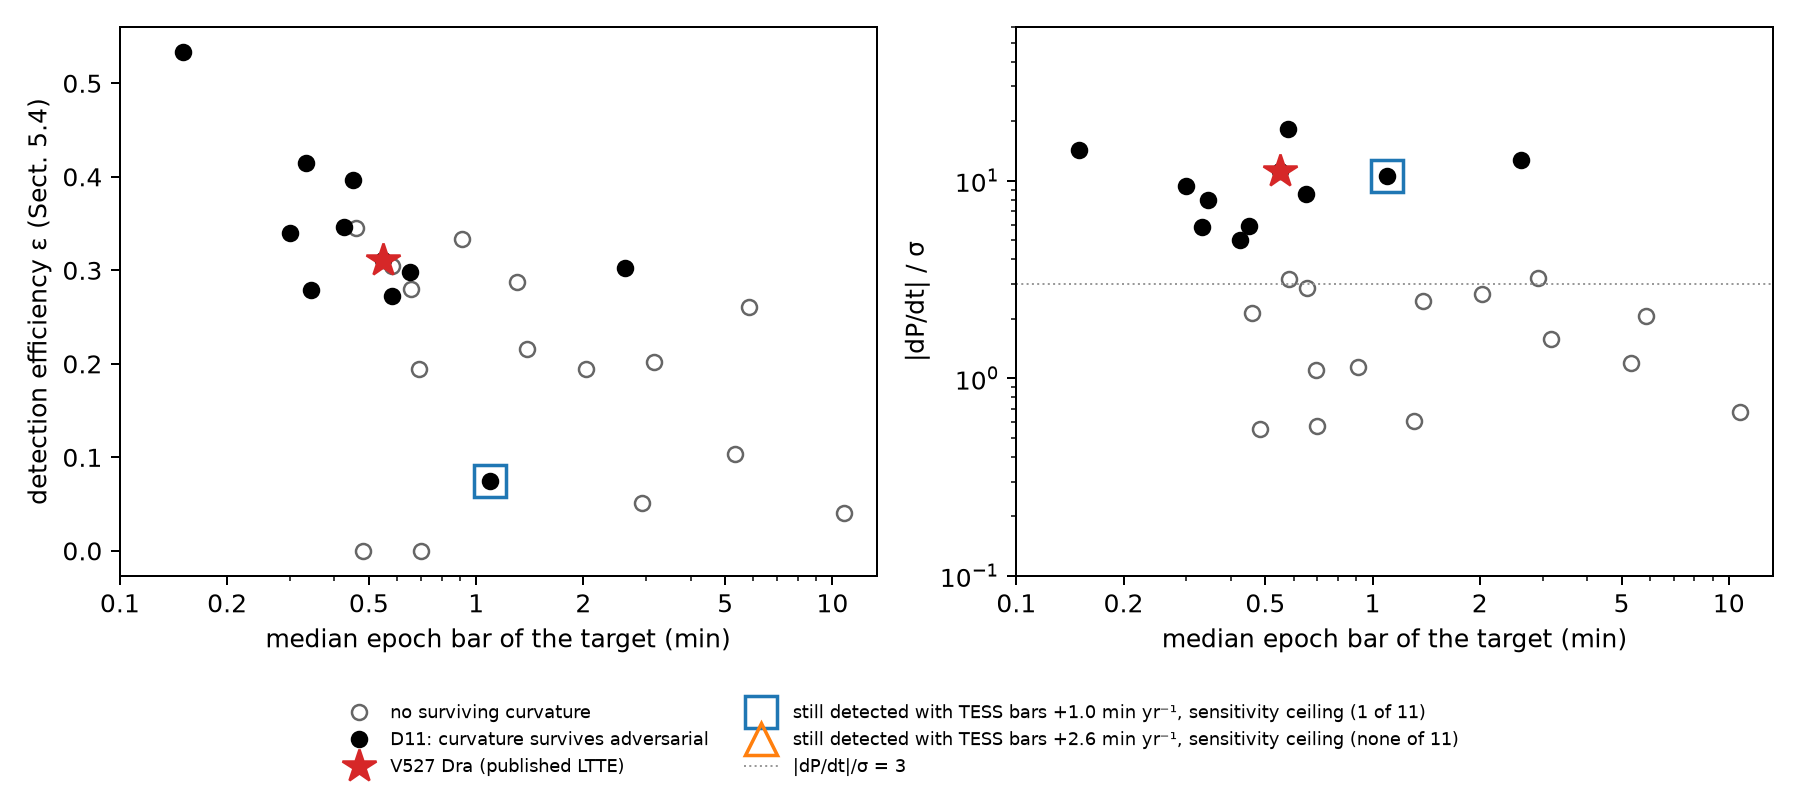
\includegraphics[width=\linewidth]{figures/fig1_barras.png}
\caption{Detection efficiency, significance and the bars. Left: the per-target detection efficiency $\varepsilon$ of Section 6 against the median epoch bar of the target; right: $|\mathrm{d}P/\mathrm{d}t|/\sigma$ against the same bar. Filled symbols are D11, the star is V527 Dra; crosses mark the detection lost when the SuperWASP bars are corrected by the measured factor (one of eleven); open squares and triangles mark the targets still detected when the TESS bars are inflated by 1.0 and 2.6 min yr$^{-1}$ (one and none); the dotted line in the right panel is $|\mathrm{d}P/\mathrm{d}t|/\sigma = 3$.}
\label{f:barras}
\end{figure*}
\begin{figure}
\centering
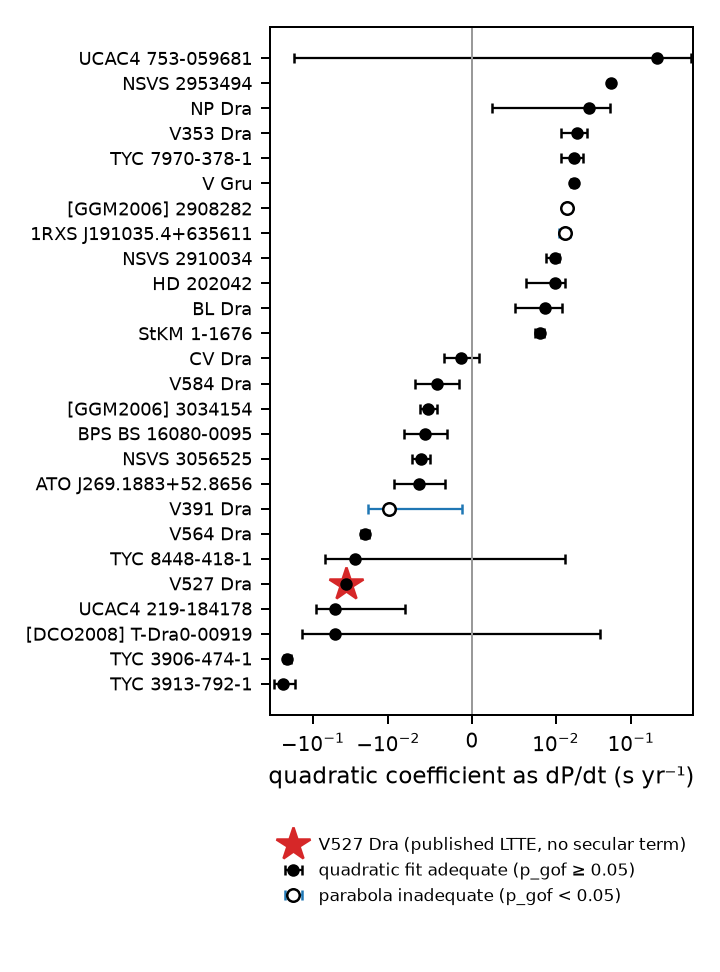
\includegraphics[width=\linewidth]{figures/fig4_dpdt.png}
\caption{Quadratic coefficients $\mathrm{d}P/\mathrm{d}t$ of the 26 targets with 1$\sigma$ bars, ordered by value; the four flagged targets ($p_{\rm gof}$ $<$ 0.05) are shown open, and V527 Dra is marked.}
\label{f:dpdt}
\end{figure}

Five remarks on the table (Fig.~\ref{f:dpdt} shows the coefficients; Fig.~\ref{f:barras} shows what the detections track). (i) In every partition the distribution is consistent with symmetry about zero: 12/14 (sign test p = 0.85), 9/13 (p = 0.52) and 7/8 (p = 1.00). (ii) The median $|\mathrm{d}P/\mathrm{d}t|$ of 0.016 s yr$^{-1}$ over all 26 is 1.9 $\times$ $10^{-7}$ d yr$^{-1}$, the order of magnitude familiar from period studies of W UMa systems; 0.009 s yr$^{-1}$ for the well-measured 15 is 1.0 $\times$ $10^{-7}$ d yr$^{-1}$. (iii) Under the earlier fixed rule $\chi^2_{\rm red}$ $\ge$ 2 the flag would have marked 7 targets instead of 4 (adding TIC 126763885, 139256217 and 424461577, whose $p_{\rm gof}$ are 0.12, 0.14 and 0.09); with 7 of 26 flagged, the chance that such a flag lands on one given target by coincidence is 27\%, a number that matters in Sect.~\ref{s:val}. (iv) Four targets have curvature at 0.01 $<$ $p_{\rm curv}$ $<$ 0.05 (TIC 126945917, 207496824, 229461186, 329289186); with 26 targets tested at the 0.05 level about one such marginal value is expected by chance, and all four fail the adversarial test in any case, so a look-elsewhere correction changes no count. (v) Two targets (TIC 224605072, 229476285) have no detection sensitivity at the amplitudes considered in Sect.~\ref{s:orb} ($\varepsilon$ = 0: their SuperWASP bars are too large for the curvature test to reject anything), so their ``no significant curvature'' is not a null result and they do not belong in the denominator of a curvature fraction; over the 24 with sensitivity the fraction is 11 of 24 (46\%, 95\% CI 28--65\%), given as a separate row of Table~\ref{t:dist}. Further rows of Table~\ref{t:dist} and the last three columns of Table~\ref{t:coef} give the detections that survive when the SuperWASP bars are corrected by the measured factor, when the TESS bars are inflated to the limit their residuals allow, under the two corrections jointly, and when the TESS bars are inflated by the between-sector drift (Sect.~\ref{s:val}).
Two sets are used by name in the rest of the note. \textbf{D11} is the eleven targets whose curvature survives the adversarial test (TIC 144194304, 198388252, 198408416, 229914020, 230386284, 232634196, 329246824, 359552377, 377253090, 392536812, 424461577); \textbf{D9} is D11 without the two flagged members (198388252, 229914020). The other two flagged targets, TIC 207496824 and 237116051, have no surviving curvature. For the two flagged members of D11 the reading is \emph{period variation detected without a determined form}; for the other two, \emph{not described by a quadratic ephemeris}; in neither case should the tabulated $\mathrm{d}P/\mathrm{d}t$ be quoted as a rate. The third column of Table~\ref{t:dist} (adequate fit and $\sigma$ $<$ 0.01 s yr$^{-1}$) contains 7 members of D9; it is a precision cut, not a third set.

\begin{figure}
\centering
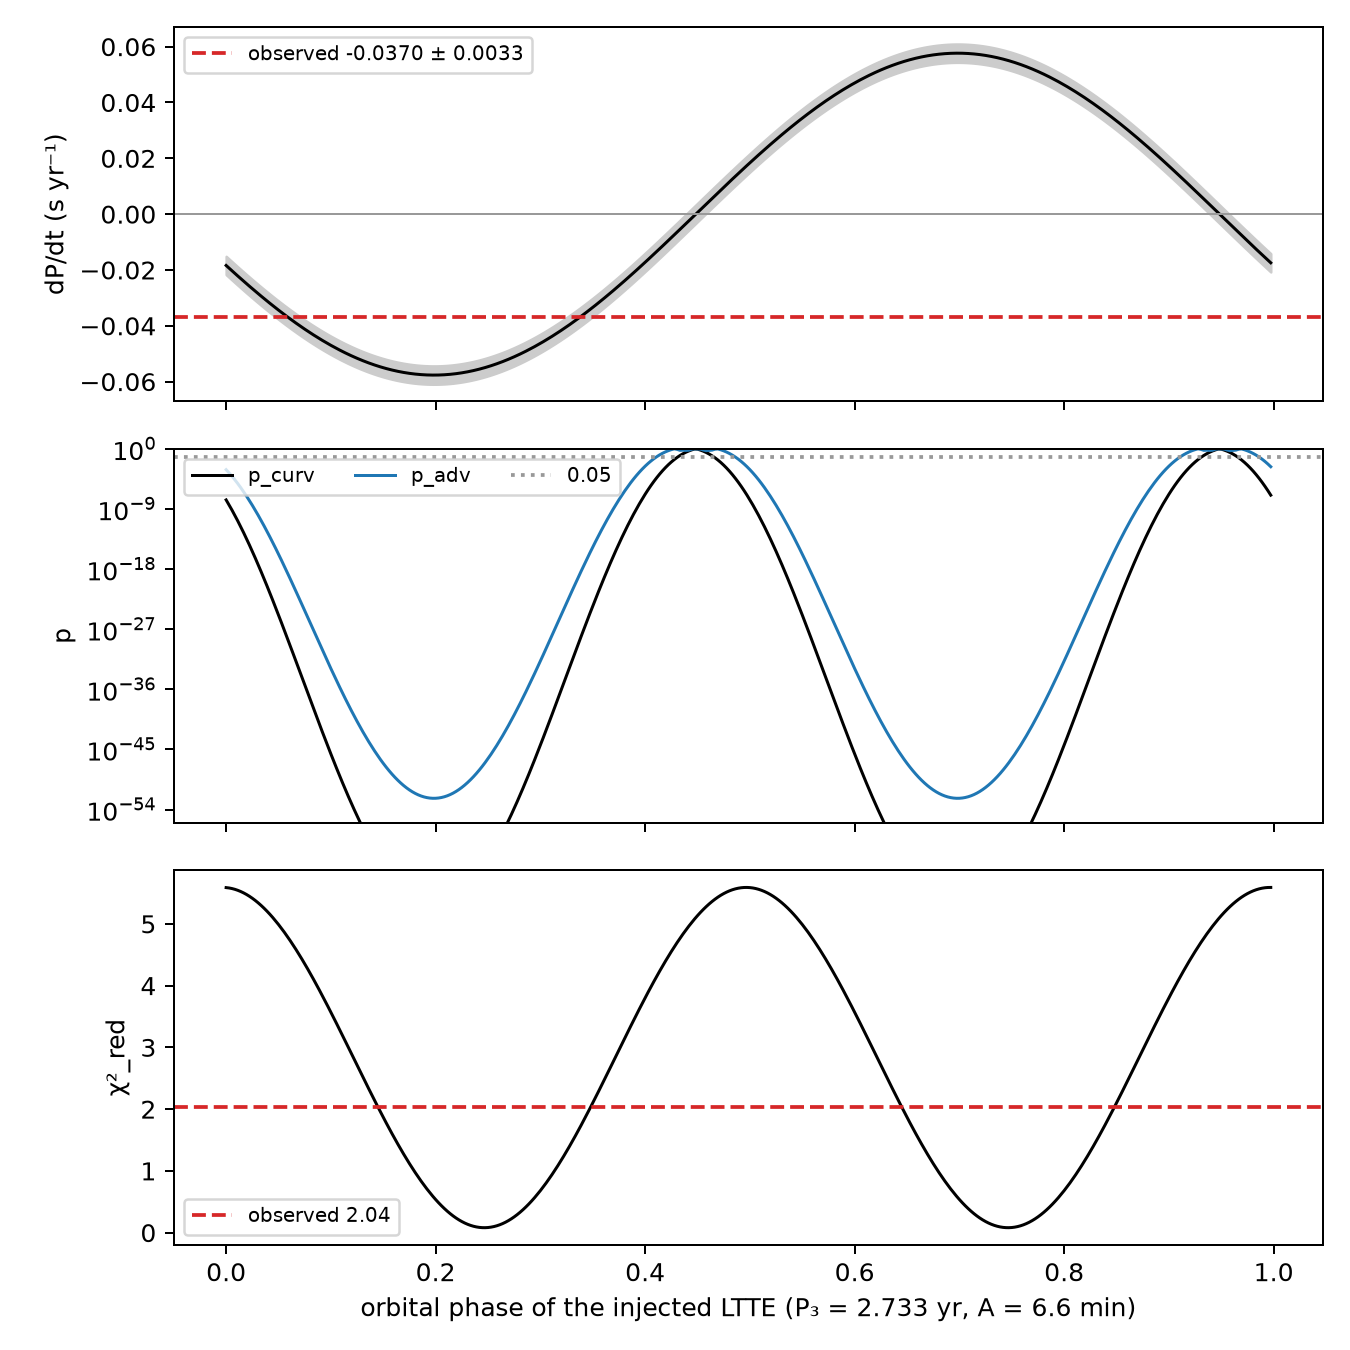
\includegraphics[width=\linewidth]{figures/fig2_v527_injecao.png}
\caption{The published LTTE orbit of V527 Dra injected on a linear ephemeris at our six epochs, over 360 orbital phases: the resulting quadratic coefficient (top), the curvature and adversarial p-values (middle) and the reduced $\chi^2$ (bottom) against phase, with the observed values marked.}
\label{f:v527}
\end{figure}
\begin{figure*}
\centering
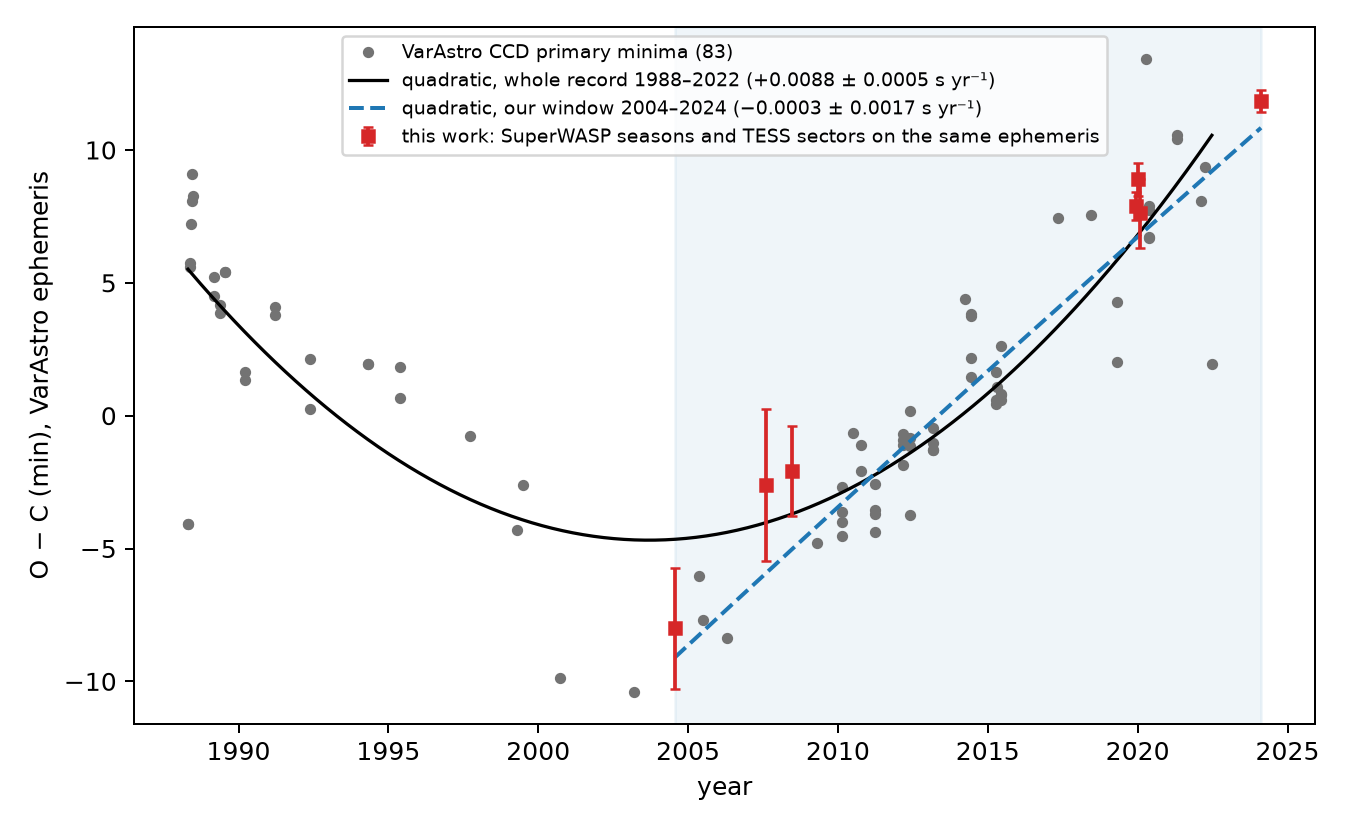
\includegraphics[width=\linewidth]{figures/fig3_cvdra.png}
\caption{CV Dra: VarAstro CCD primary minima 1988--2022 with the quadratic fitted to the whole record and the one fitted to our 2004--2024 window, and our epochs placed on the same ephemeris.}
\label{f:cvdra}
\end{figure*}
\section{Validation and external confrontation}\label{s:val}
The control target (TIC 142874476), on which the chain was developed, was re-run before and after every change reported in this version and reproduced each time; its component-by-component record is internal quality assurance and is given in Appendix~\ref{a:B}.
\textbf{Period ladder.} The ladder returns epochs and residuals in the caller's order. This was a latent defect: an earlier version returned them in internal time order, and unsorted input produced cycle numbers assigned to the wrong sectors --- caught only because the resulting $\mathrm{d}P/\mathrm{d}t$ of $-$24\,122 s yr$^{-1}$ is physically impossible; a milder scramble would have looked like mass transfer. The $|\mathrm{d}P/\mathrm{d}t|$ $>$ 10 s yr$^{-1}$ guard of Sect.~\ref{ss:escada} exists because of it. The tolerance rule of Sect.~\ref{ss:escada} (the larger of 3 min and 3$\times$ the median epoch uncertainty) was introduced after the main batch, which ran with a fixed 3 min; re-running all 26 targets under the rule reproduces every tabulated value (1\,024 fields compared across the 26 per-target records; only the wall-clock time differs).
\textbf{Error calibration.} The reduced $\chi^2$ of the quadratic fit is the check that the assigned errors describe the residuals. With formal errors it had median 6.35 (25th--75th: 2.08--37.5), was below 2 for only 8 of 31, and left maximum quadratic residuals of 4.4 min (median) to 18 min (75th percentile) against bars of 0.4--0.7 min: not even the more complex model explained the residuals, which locates the problem in the denominator, not the model. With errors from the data (Sect.~\ref{ss:barras}) it has median 1.41 --- and earlier versions of this note read that as validation. It is not: with 1--4 degrees of freedom the median of $\chi^2/\nu$ under correct bars is well below 1 (0.45 at $\nu$ = 1), and for the actual distribution of degrees of freedom of the 26 (five at 1, eight at 2, six at 3, seven at 4) the expected median is 0.73, with a 95\% range of the median of 0.43--1.15 (20\,000 simulations; \texttt{src/reinflar\_tess\_26.py --resumo}). A median of 1.41 has probability 0.0016 under correct bars. The aggregate says the same: $\Sigma\chi^2$ = 128.6 for 67 degrees of freedom, reduced $\chi^2$ 1.92 (p = 9 $\times$ $10^{-6}$); median and aggregate imply the same bar factor, $\sqrt{1.92}$ = 1.39, and the agreement is informative because the aggregate is dominated by the two worst-fitting flagged targets and the median is not.
\textbf{Which bar is too small.} A global factor says the total variance is underestimated, not where. The residuals of the quadratic fits, normalised by the bar of each epoch and corrected for leverage --- with three parameters on 4--7 points, E[r$^2$/$\sigma^2$] = 1 $-$ h, and h reaches 0.6 for the TESS epochs --- were summed separately over the 84 TESS and 61 SuperWASP epochs of the 26 targets (\texttt{src/qual\_barra\_26.py}; expectation written before running: excess in TESS). The result is the opposite. The SuperWASP epochs give $\Sigma z^2$ = 95.6 against 35.0 expected, a variance factor of 2.73 ($\chi^2$ interval 1.79--4.64; bootstrap over targets 1.34--4.71), i.e. bars 1.65 (1.34--2.15) times too small; the TESS epochs give 33.0 against 32.0, a variance factor of 1.03 (0.67--1.81; 0.43--1.81), i.e. bars 1.02 (0.82--1.35) times too small --- the two numbers are in different units and are given in both for both sets. The mean leverage is 0.62 for the TESS epochs and 0.43 for the SuperWASP ones: the test retains 38\% of the TESS variance and 57\% of the SuperWASP variance. Of the total excess of +61.6, +60.5 is in SuperWASP. The ``term whose true size is unknown and is at least 0.78 min'' of Sect.~\ref{ss:vies} now has a size. The test is asymmetric and that must be said: it has power for SuperWASP, whose epochs sit at the end of the lever, and little for TESS, whose four epochs are fitted by three parameters --- what the parabola absorbs does not appear as a residual, and the TESS-internal structure is exactly what was called curvature. A TESS excess at the between-sector scale is therefore not excluded by this test; it is only not required by it. Whether the leverage biases the two factors was measured rather than asserted (\texttt{src/vies\_alavanca\_26.py}; simulation on the 26 actual designs, 2\,000 realisations per case): for errors that scale the bars, the estimator is unbiased in both sets --- recovered variance factors within 2\% of the truth for TESS factors of 1, 1.34 and 2 and SuperWASP factors of 1, 1.65 and 2.15, with no leakage between sets --- so 2.73 and 1.03 are estimates, not a floor and a ceiling. For coherent timing structure at the TESS epochs that lies \emph{outside} the parabola (a sinusoid of period 2 yr), the TESS factor responds first and strongly (1.25, 3.3 and 10 for amplitudes of 1, 3 and 6 min) and the SuperWASP factor only weakly (1.01, 1.23, 1.89): the measured TESS factor of 1.03 ($\le$ 1.81) bounds such structure at about 1 min, and the SuperWASP factor of 2.73 cannot be a leak from it. What the test cannot see is structure \emph{inside} the parabola --- a drift that is linear or quadratic over the four TESS epochs is absorbed into the coefficient --- and that is the blindness that matters, because it is exactly the between-sector drift of the secondaries.
\textbf{How much of the SuperWASP excess could be signal.} An undersampled third-body orbit is exactly the structure that the four TESS epochs absorb into the parabola and the SuperWASP seasons, 12--16 yr away, do not: it appears as SuperWASP residual excess, and V527 Dra shows the sample contains at least one. Whether the factor of 2.73 is bar error or partly that signal was measured (\texttt{src/estrutura\_swasp\_26.py}; expectation written and committed before running: a SuperWASP factor of 1.10--1.30 at f = 0.24) by injecting the declared orbit population of Sect.~\ref{s:orb} into the 26 designs with correct bars, at all epochs, with occurrence f, and reading the two factors. The expectation was wrong. At f = 0.24 the population alone gives a SuperWASP factor of 1.73 on average (median 1.27; 2.5--97.5\%: 0.70--5.93; the distribution is heavy-tailed because a few large, long-period orbits dominate) --- 42\% of the measured excess on average --- but it also gives a TESS factor of 1.58 (median 1.37; 0.68--3.72), because orbits with $P_3$ shorter than the 4-yr TESS span are not parabolic over the four sectors. The measured TESS factor is the lock: among the realisations compatible with it (TESS $\le$ 1.03, 22\% of them at f = 0.24) the SuperWASP factor averages 1.37 (95th percentile 2.75); among those compatible with its 95\% limit (TESS $\le$ 1.81, 73\%) it averages 1.58 (95th percentile 3.60). For orbits alone to produce 2.73 the in-window fraction would have to be 0.59, and the TESS factor would then be 2.4. The reading is therefore: the SuperWASP excess is part bar and part astrophysics. The factor is a ratio of variances and independent contributions add, so the orbits' 1.37 contributes an excess of 0.37 and the bar-only factor is $\sqrt{2.73 - 0.37}$ = 1.54 (1.47 with the conditional at the 95\% TESS limit, 1.58; and $\sim$1.0 --- no bar correction at all --- at the 95th percentile of the conditional, where the orbits alone reach the whole excess). The bar factor is therefore 1.0--1.65 with 1.54 central, and \textbf{the correction by 1.65 is a ceiling on the bar error, and the joint correction below is a ceiling as well.} The same simulation turns the TESS factor into an internal constraint on the in-window tertiary fraction, independent of Tokovinin et al.: for the declared population, the probability that the TESS factor is as low as the measured 1.03 is 0.39 at f = 0.10, 0.23 at 0.24, 0.17 at 0.30, 0.09 at 0.41, 0.06 at 0.50, 0.014 at 0.70 and 0.004 at 1.0 (\texttt{estrutura\_swasp\_26\_grade\_f.parquet}). The 5\% crossing lies between the grid points 0.50 (0.058) and 0.70 (0.014), at f $\approx$ 0.52 by interpolation in log p; the TESS residuals alone therefore exclude f $\\gtrsim$ 0.5 at 95\%, disfavour 0.41, and are compatible with 0.24. This is a one-sided tail test: p decreases monotonically with f, so it always prefers a smaller f and cannot identify a central value --- f = 0.10 has p = 0.39 and is not thereby preferred. It bounds the fraction from above and says nothing against 0.24; the external fraction supplies the central value and the internal test the ceiling. A population of larger amplitudes would tighten the bound. The counts are bracketed by runs already made: the SuperWASP factors 1.34 and 1.65 both leave 10 of the 11 detections, so a bar-only correction of 1.4 would too; what the ceiling costs is the precision of TIC 232634196 and the one detection (TIC 359552377) that rested on the seasons.
\textbf{SuperWASP bars corrected by the measured factor.} Every SuperWASP epoch bar was multiplied by 1.65 (and by the ends of the interval, 1.34 and 2.15), the TESS bars left unchanged, and the stored epochs refitted with the same tests (\texttt{src/reinflar\_swasp\_26.py}; expectation written before running: the median reduced $\chi^2$ near 0.73, the TESS-internal detections unchanged, TIC 232634196 surviving at the central factor). The median reduced $\chi^2$ becomes 0.63 (0.86 and 0.42 at the interval ends) and the aggregate 1.01 (1.28, 0.79). The measured factor sits where the residuals want it (a median of 0.63 has probability 0.27 of being this low under correct bars, 0.86 has 0.25 of being this high); the upper end of the interval does not --- a median of 0.42 has probability 0.019 under correct bars, so $\times$2.15 over-inflates, which is information about the interval and not only a sensitivity run. \textbf{Ten of the eleven detections stand} (10 at 1.34, 8 at 2.15); the one that falls at the central factor is TIC 359552377, whose curvature rested on the SuperWASP seasons ($p_{\rm adv}$ 0.36 after correction), and TIC 229914020 and 377253090 fall only at the upper end. No new detection appears. The per-target efficiency of Sect.~\ref{s:orb} becomes $\Sigma\varepsilon$ = 5.7 (from 6.7). This is the correction the data support, and it does not remove the detections: they are carried by the TESS epochs.
\textbf{The TESS inflation the residuals allow, and the joint corrections.} The TESS residual factor of 1.03 has a 95\% upper limit of 1.81 in variance, i.e. bars up to 1.34 times too small; that is the only TESS inflation the data oblige one to consider, and it was run, alone and together with the SuperWASP correction (\texttt{src/reinflar\_conjunto\_26.py}; expectation written and committed before running: 10--11 of 11 alone, 9--10 jointly, 0--1 under the joint ceiling). Alone, TESS $\times$1.34 leaves 10 of the 11 (TIC 359552377 falls at the adversarial test), with the median reduced $\chi^2$ at 1.30 because the SuperWASP excess is untouched. \textbf{SuperWASP $\times$1.65 with TESS $\times$1.34 --- the conservative correction the data support --- leaves 8 of the 11} (TIC 229914020, 359552377 and 377253090 fall), with the median reduced $\chi^2$ at 0.55 (probability 0.13 of being this low under correct bars --- consistent with correct bars, on the over-corrected side, as it should be when the TESS factor is a limit and not an estimate) and the aggregate at 0.79; $\Sigma\varepsilon$ = 5.1. SuperWASP $\times$1.65 with TESS +1.0 min yr$^{-1}$ --- the conservative ceiling --- leaves one (TIC 232634196, $-$0.210 $\pm$ 0.035 s yr$^{-1}$), with the median at 0.32 (probability 0.002: over-inflated, as a ceiling should be). The joint runs are needed because in a three-parameter fit on 4--7 points the two corrections are not independent or additive: the SuperWASP correction alone removes one detection and the TESS limit alone removes one, the two together remove three.
\textbf{TESS bars at the between-sector scale: a sensitivity test with a ceiling.} The secondary-minimum test below finds the secondary drifting with respect to the primary by 1.0--2.6 min yr$^{-1}$ between sectors in five of 24 targets. The TESS bar of Sect.~\ref{ss:barras} is the dispersion between the two halves of a sector, a within-sector quantity over $\sim$13 d, and cannot contain such a drift; the residual test above cannot see it either. Whether the primary epochs wander at a comparable rate is therefore untested, and the question matters because the detections are TESS-internal. The test that was run (\texttt{src/reinflar\_tess\_26.py}; expectation written and committed before running) inflates every TESS epoch bar of a target in quadrature by d $\times$ L, with d = 1.0 or 2.6 min yr$^{-1}$ (the extremes of the measured secondary drift; no central value) and L the target's own TESS lever (median 4.2 yr), giving median TESS bars of 4.2 and 10.9 min; the SuperWASP bars are unchanged; the stored epochs are refitted (linear and quadratic, curvature and adversarial tests, goodness of fit, the TESS-only period and the cycle-count criterion) and the efficiency of Sect.~\ref{s:orb} is re-measured. This is an extrapolation of a drift measured on the secondary in five targets to the primary epochs of all 26, and 1.0 min yr$^{-1}$ is a ceiling, not an estimate: the TESS residuals do not ask for it, and an earlier version of this note, which called the 1.0 min yr$^{-1}$ bars ``calibrated'' because they brought the median reduced $\chi^2$ to 0.73, was wrong --- that coincidence came from re-weighting (larger TESS bars let the parabola reach the SuperWASP seasons, reducing \emph{their} residuals), not from correcting the bar the residuals identify. The expectation was that 6--9 of the eleven would survive at 1.0 min yr$^{-1}$ and 3--6 at 2.6. The result: \textbf{at 1.0 min yr$^{-1}$, one of the eleven survives (TIC 232634196); at 2.6, none} (Table~\ref{t:coef}, last two columns; Table~\ref{t:dist}; Fig.~\ref{f:barras}). The cycle count across the gap stays unambiguous in every case ($\sigma_P$ $\times$ N $\le$ 0.04). The response is not monotonic, and ``no new detection appears'' would misdescribe it: at 1.0 min yr$^{-1}$ four targets have $p_{\rm curv}$ $<$ 0.05 (TIC 232634196, 237116051, 359552377, 392536812) and only the first passes the adversarial test; two targets become \emph{more} significant in curvature as the bars grow --- TIC 237116051 from $p_{\rm curv}$ 0.39 to 0.001 and TIC 198388252 from 0.11 (at 1.0) to 0.002 (at 2.6) --- because the weight migrates to the SuperWASP seasons and the fit changes, and both fail the adversarial test. A reading, generated after the fact and labelled as such: inflating the TESS bars does not only remove detections, it redistributes the weight between the two time-scales, and for those two targets a long-baseline curvature that the TESS weight suppressed emerges when the archival seasons dominate. The reading is not delivered by the test --- both targets fail the adversarial test, and the same redistribution story would fit any target whose weights migrate --- so it is a hypothesis about where each target's curvature lives, not a result. Ten of the eleven detections are therefore structure within the five years of TESS, and the note cannot certify that structure as period change against between-sector timing noise of the size the secondaries show: the within-sector bars do not contain it, and the residual test cannot detect it.
\textbf{TIC 232634196: the one detection tested against the bar the data say is wrong.} TYC 3906-474-1 (Tmag 9.9, P = 1.2511 d, catalogue morphology 0.66), coefficient $-$0.213 $\pm$ 0.013 s yr$^{-1}$ with the original bars. Unlike the other ten, its curvature is carried by the 20-yr lever: on the linear ephemeris the three SuperWASP seasons sit at $-$116, $-$84 and $-$94 min, and the quadratic through them predicts the TESS-internal change that is observed (quadratic residuals of the four TESS epochs within $\pm$0.7 min). The spread of the three seasons, 32 min, is not a test of them: the 11.5-min bars are built from that same between-season dispersion, so the spread is 2.8$\sigma$ by construction. What sustains the lever is the \emph{mean} of the three seasons, $-$98 min from the linear ephemeris, and that is why multiplying the bars by 1.65 (to 19 min) barely moves the coefficient. Because the SuperWASP bars are the ones the residuals identify as too small, this is the only detection that is tested against the correction the data support: with those bars multiplied by 1.65 it gives $-$0.214 $\pm$ 0.020 s yr$^{-1}$ ($p_{\rm curv}$ and $p_{\rm adv}$ $<$ $10^{-4}$), and it survives at 2.15 as well ($-$0.214 $\pm$ 0.026). It also survives the TESS sensitivity test at 1.0 min yr$^{-1}$ ($-$0.200 $\pm$ 0.031) and fails only at 2.6 (adversarial). The cycle count across the gap is unambiguous ($\sigma_P$ $\times$ N = 0.014), there is no VarAstro record and no literature on the star. Whether the primary and the secondary move together or in opposition was measured on the same 20-yr linear ephemeris of the primaries (\texttt{src/caso\_232634196.py}; the expectation was declared as not blind, because the stored numbers were already in view): the change from the 2019--2020 sectors to sector 75 is $-$6.9 $\pm$ 0.9 min for the primary and $-$15.8 $\pm$ 1.5 min for the secondary --- same sign, both significant. That excludes the anti-correlated signature of apsidal motion, and it is where the conclusion stops: the common mode, $-$6.9 min, is the \emph{smaller} of the two terms, and the differential, $-$9.0 $\pm$ 1.7 min, the larger. A period change plus a differential drift reproduces the observation; so does a spot pattern that affects the two minima unequally. The data do not separate the two hypotheses. The reference matters and is stated: a linear ephemeris fitted to the TESS epochs of both minima at once would split the differential drift between them by construction and read ``opposition'' for any target; the reference used is the ephemeris against which the curvature was claimed. What the note can say about this star is therefore: a curvature over 16--20 yr carried by the archival lever, which survives the correction of the archival bars and the TESS sensitivity test at its lower value, whose secondary moves in the same direction as its primary, and whose common-mode change is smaller than the differential one; a third-body orbit is not excluded (Sect.~\ref{s:orb}). It is one object; it is not developed further here.
\textbf{Published work on the 26.} Each target was cross-matched by position with SIMBAD (5\arcsec; 26 of 26 matched, median 10 references per object, minimum 1, maximum 33) and with the VarAstro star catalogue (1\arcmin; Paschke \& Brát 2006), the successor of the O$-$C Gateway that inherited its minima database (13 of 26 have an entry; 12 have at least one primary minimum; 6 have $\ge$ 4 CCD primary minima, spanning 7.7--34 yr). The SIMBAD bibliographies are catalogue-scale except for five object-scale papers ($\le$ 10 objects): TIC 424461577 = V527 Dra (see below); TIC 144194304 = V Gru (Tanrıver et al. 2023), whose timing analysis covers 2018--2020 only and reports a linear ephemeris; TIC 229687624 = CV Dra (IBVS 3213, 1988), light curves and preliminary elements; TIC 230386284 (Pyatnytskyy 2020), photometry only; and TIC 126945917 = HD 202042, one of five oscillating Algols in Pawar et al. (2026), whose O$-$C analysis uses TESS sectors 1, 27, 28 and 68 only, attributes an anti-correlation between primary and secondary timings to spots, and states that with data spanning so short a time no conclusion on the mass-transfer rate can be drawn --- no $\mathrm{d}P/\mathrm{d}t$ is reported (ours: +0.0084 $\pm$ 0.0035 s yr$^{-1}$, no significant curvature). No target has a published $\mathrm{d}P/\mathrm{d}t$. The subpopulation is more studied than we anticipated: the expectation written before the query was $\le$ 5 targets in the VarAstro database and $\le$ 2 with an object-scale paper.
\textbf{V527 Dra: a false positive of secular curvature that passes every internal test.} The eclipse-timing analysis of V527 Dra (Čeki et al. 2024; 1\,832 timings including 34 from SuperWASP) is a light-travel-time orbit with $P_3$ = 2.733 $\pm$ 0.005 yr and semi-amplitude 6.6 min, \emph{with no secular term}; the star is also one of the eleven objects SIMBAD links to the TESS full-frame-image timing study of Marcadon \& Prša (2024), which reports ten new triple candidates. Our chain, with six epochs and no access to any of those timings, returned $\mathrm{d}P/\mathrm{d}t$ = $-$0.0359 $\pm$ 0.0038 s yr$^{-1}$ with $p_{\rm curv}$ $\approx$ $10^{-21}$, $p_{\rm adv}$ $\approx$ $10^{-14}$ and $p_{\rm gof}$ = 0.089: a curvature detection that survives the adversarial test and whose quadratic fit is not rejected, in a system whose published O$-$C has no secular term. An earlier draft of this note, using the fixed $\chi^2_{\rm red}$ $\ge$ 2 flag, had marked this target ($\chi^2_{\rm red}$ = 2.18) and described the mark as a blind validation of the flag; under the degrees-of-freedom-aware criterion of Sect.~\ref{ss:testes} the mark does not exist, and with 7 of 26 targets flagged under the old rule the coincidence had a 27\% prior probability in any case. That statement is withdrawn. What remains is the stronger and less comfortable fact: \textbf{the one target with an external record of a cyclic O$-$C passed all three internal tests, and it is therefore a member of D9, the cleanest set this note has.} The denominator for a false-positive rate is not nine: only two members of D9 have an external record long enough to test the secular reading, V527 Dra and V564 Dra (below), and the other seven are untested, not confirmed. Of the two testable, one fails (V527 Dra, published cyclic O$-$C without a secular term) and the other disagrees outside our window (V564 Dra): 1 of 2, 95\% Wilson interval 9--91\%, with seven that cannot be tested. Less precise than a rate, and what the data support. An earlier version of this paragraph quoted a rate of one in nine ``verified against the literature''; that implied a test that does not exist for seven of the nine.
The mechanism is measurable. Six epochs over 15.7 yr sample a 2.73-yr cycle at essentially three phases (2008.4--2008.6, 2019.9--2020.1, 2024.1), and a three-parameter parabola passes through three groups, leaving only the intra-group structure as residual: this is why the goodness-of-fit test does not reject the parabola ($p_{\rm gof}$ = 0.089; $\chi^2_{\rm red}$ 2.18 against an expected median of 0.79 at 3 degrees of freedom, i.e. 2.8 times the expectation but within the tail), whereas a 6.6-min signal against sub-minute bars would give $\chi^2_{\rm red}$ of tens if the cycle were not absorbed. With the SuperWASP bars corrected by the measured factor the target still passes all three tests ($\chi^2_{\rm red}$ 1.96, $p_{\rm gof}$ 0.12). The published orbit (circular, A = 6.6 min, $P_3$ = 2.733 yr) was injected on an exactly linear ephemeris at our six epoch times with our bars, over 360 orbital phases (\texttt{src/v527\_ltte.py}; expectation written before running; Fig.~\ref{f:v527}). The quadratic coefficient ranges from $-$0.058 to +0.058 s yr$^{-1}$ ($|\mathrm{d}P/\mathrm{d}t|$ $\ge$ 0.036 at 57\% of phases), $p_{\rm curv}$ $<$ 0.05 at 92\% of phases, $p_{\rm adv}$ $<$ 0.05 at 83\%, $\chi^2_{\rm red}$ median 2.86 (below 3 at 52\% of phases, maximum 5.6); 26 of the 360 phases return a coefficient within 0.005 s yr$^{-1}$ of the observed one, with $\chi^2_{\rm red}$ between 1.3 and 5.2. The observed outcome is a typical product of a parabola over an undersampled third-body cycle. \textbf{The adversarial test shifts epochs, not phases, and does not protect against it: 83\% of phases survive.} Any triple system in the sample with an outer period shorter than the baseline and longer than a sector passes every internal test here and fails only an external one. Sect.~\ref{s:orb} asks how many such systems the sample is expected to contain.
\textbf{Independent minima.} For the six targets with $\ge$ 4 CCD primary minima in the VarAstro database, the same quadratic ephemeris was fitted to those minima alone (VarAstro's own ephemeris for the cycle count; unweighted least squares; per-point error from the MAD of the quadratic residuals; primary minima only, CCD/photoelectric only). One was excluded for a period-convention discrepancy that anyone repeating the cross-match will meet: for V391 Dra (TIC 237116051) VarAstro adopts half the catalogue period (1.2315 d against 2.4629 d), and 5 of its 7 ``primary'' minima fall at phase 0.5 of the catalogue ephemeris --- they are secondary minima under the convention of Table~\ref{t:coef}, and the two sets do not time the same event. Over the whole VarAstro record, 2 of the remaining 5 agree with Table~\ref{t:coef} within 2$\sigma$ (BL Dra = TIC 229461186, z = +1.0; V353 Dra = TIC 207496824, z = $-$1.0) and 3 do not: CV Dra (TIC 229687624; record 1988--2022, 83 minima: +0.0088 $\pm$ 0.0005 s yr$^{-1}$ against our $-$0.0006 $\pm$ 0.0021, z = $-$4.3), V564 Dra (TIC 329246824; 1999--2025, 10 minima: $-$0.0066 $\pm$ 0.0011 against $-$0.0199 $\pm$ 0.0018, z = $-$6.4) and V527 Dra (the published LTTE system, z = $-$6.5). Restricting the VarAstro fit to the baseline of our own epochs ($\pm$0.5 yr) changes the picture: CV Dra $-$0.0003 $\pm$ 0.0017 (z = $-$0.1), V564 Dra $-$0.0130 $\pm$ 0.0042 (z = $-$1.5), BL Dra +0.0082 $\pm$ 0.0098 (z = +0.1), V353 Dra $-$0.02 $\pm$ 0.13 (z = +0.3) --- 4 of 4 (V527 Dra has 2 in-window minima). At the level of the data, placing our epochs on VarAstro's ephemeris next to the CCD minima taken within one year gives, for the SuperWASP era (the independent one; 2 comparisons, both CV Dra): $-$7.1 $\pm$ 2.3 vs $-$6.9 min and $-$1.2 $\pm$ 1.2 vs $-$4.8 $\pm$ 1.9 min; for the TESS era, 12 of 13 within 2$\sigma$ with rms z = 1.16 (VarAstro minima after 2018 may themselves derive from TESS, so this is consistency, not independence). The median offset, +0.5 min, is of the order of the HJD\_UTC/BJD\_TDB conversion and is not interpreted.
The window-restricted test is the demonstration: it is not that our measurement disagrees with the archive's, it is that the two fits measure different windows of a curve that is not polynomial --- same window, 4 of 4 agree; whole record, 2 of 5 (Fig.~\ref{f:cvdra}). The epochs agree and the coefficients do not, because the O$-$C is not a parabola over the longer record: the VarAstro O$-$C of CV Dra runs from +5 min (1988) through $-$10 min (2002) to +8 min (2022), and its quadratic residuals reach 9.6 min against an intra-year scatter of 2.4 min. A quadratic fitted over 16--20 yr returns the local coefficient over that baseline, and the two targets with longer external records show that it does not extrapolate.
\textbf{Secondary minima.} Apsidal motion in an eccentric orbit produces a spurious quadratic in the primary alone, with the secondary moving the opposite way; a secular $\mathrm{d}P/\mathrm{d}t$ moves both together. The secondary epoch was measured in every TESS sector of the 26 with the same estimator, the catalogue seed shifted by P/2, the same trapezoid and the same halves-dispersion bar (\texttt{src/secundarios\_26.py}; expectation written before running: most secondaries measurable, 0--2 targets with a significant differential drift, up to 5 with no measurable secondary). The quantity tested is d = t\_sec $-$ t\_prim $-$ P/2 per sector, and its drift between the first and last sector (median lever 4.2 yr within TESS). All 26 secondaries were measurable; for two of the long-period targets (TIC 139256217, 359552377) the bar on d exceeds 10 min and the test is uninformative, leaving 24. In 5 of the 24 the secondary sits more than 2$\sigma$ from phase 0.5 (TIC 126763885, 224605072, 229914020, 232634196, 329246824), which is a statement about eccentricity or asymmetry, not about period change. In 5 of the 24 the differential drift is significant at $>$ 2$\sigma$ --- more than the 0--2 expected: TIC 229476285 ($-$1.50 $\pm$ 0.38 min yr$^{-1}$), 229914020 (+2.59 $\pm$ 0.29; flagged), 232634196 ($-$1.80 $\pm$ 0.50), 329289186 (+2.41 $\pm$ 0.52) and 390021728 (+0.67 $\pm$ 0.33). None of the four targets with P $>$ 2 d and an informative secondary shows a drift, so the eccentric-orbit confounder is not detected where it was expected; the drifts occur in systems with P = 0.3--1.25 d, where migrating spots are the usual cause of differential primary/secondary timing. On the one target where a published primary/secondary comparison exists, HD 202042 (TIC 126945917), Pawar et al. (2026) report an anti-correlation within TESS sectors; our sector-to-sector drift for the same target is +0.50 $\pm$ 0.49 min yr$^{-1}$, not significant, so our data do not confirm their effect at the level our bars allow. Of the eleven detections of D11, two are affected, and they are one story. TIC 229914020 has the largest differential drift of the sample (+2.59 $\pm$ 0.29 min yr$^{-1}$, 9$\sigma$), is flagged by the goodness-of-fit test, and is in D11: its curvature, its bad fit and its drifting secondary are three views of the same non-quadratic timing behaviour, and the target belongs to none of the categories that read as period change. TIC 232634196, in D9, has a differential drift of $-$1.8 $\pm$ 0.5 min yr$^{-1}$ measured over 4.2 yr, i.e. 7.5 min within the TESS span; extrapolated linearly over the 20-yr baseline --- an illustration, since the drift was measured on a fifth of that interval --- it would amount to 36 min against a quadratic excursion of 208 min, so the secondary shares most of that curvature, not necessarily all of it. The primary/secondary test therefore qualifies two of the eleven; it does not bear on the third-body mechanism of Sect.~\ref{s:orb}, which moves both minima together.
The excess itself --- five drifts against 0--2 expected --- is the measurement behind the TESS sensitivity test above: a spot-driven drift of 1--2.6 min yr$^{-1}$ between sectors years apart is invisible to a within-sector bar and to the residual test, and when a drift of that size is added to the TESS epochs, ten of the eleven detections disappear. Whether the primaries drift as the secondaries do is the question the data leave open.

\section{How many of the curvature detections are expected to be third-body orbits?}\label{s:orb}
The V527 Dra result turns a case into a rate question, with two ingredients that must not be confused: how often a close binary has a tertiary with an outer period inside the window where undersampling produces curvature, and how often such an orbit, sampled at a target's actual epochs with its actual bars, produces a detection by the tests of Sect.~\ref{ss:testes}.
\textbf{Detection efficiency per target.} The $\varepsilon$ = 0.83 of Sect.~\ref{s:val} was measured for one orbit and one sampling pattern and cannot be transferred. It was measured on each target (\texttt{src/epsilon\_26.py}; expectation written and committed before running) by injecting a declared population of circular tertiary orbits --- $P_3$ log-uniform in 0.1--20 yr, masses and inclination as in Appendix~\ref{a:C}, amplitude from Kepler's third law, which reproduces the published 6.6 min of V527 Dra --- on an exactly linear ephemeris at the real epoch times with the real bars, 2\,000 orbits per target, each judged by the curvature and adversarial tests. $\varepsilon$ ranges from 0.00 to 0.53 (mean 0.26), is set by the size of the bars and not by the sampling pattern (Appendix~\ref{a:C}), and sums to $\Sigma\varepsilon$ = 5.1 over the 26 under the conservative joint correction of Sect.~\ref{s:val} (5.7 with the SuperWASP bars alone corrected, 6.7 with the original bars; 21.6 is the ceiling for orbits all as favourable as V527 Dra's). It treats orbit and secular term as exclusive.
\textbf{In-window tertiary fraction.} From Table~\ref{t:barras} of Tokovinin et al. (2006; VizieR J/A+A/450/681), of the 42 solar-type spectroscopic binaries with inner period below 3 d, 10 have their closest tertiary at an outer period of 0.1--20 yr: f = 0.24, 95\% Wilson interval 0.13--0.39 (0.41 under the hypothesis that all the incompleteness the paper corrects for lies inside the window). The TESS residuals of this sample give an independent constraint (Sect.~\ref{s:val}): for the declared orbit population they are compatible with f = 0.24 (probability 0.23 of a TESS factor as low as measured), disfavour 0.41 (0.09) and exclude f $\\gtrsim$ 0.5 (the 5\% crossing is at f $\approx$ 0.52), so the external fraction and the internal bound agree, and the 0.41 hypothesis is the upper edge of what the data allow rather than a live alternative; the internal test is one-sided and bounds f from above only, which is why the central value is taken from Tokovinin et al. and not from it. Survey-detected fractions (Borkovits et al. 2016; Hajdu et al. 2019; Marcadon \& Prša 2024) are floors already convolved with each survey's efficiency and are not multiplied by $\varepsilon$ (Appendix~\ref{a:C}). The transfer to this sample --- six targets with P $>$ 2 d, five detached --- is asserted, not demonstrated.
\textbf{The number.} Under the conservative joint correction, the expected number of the eight surviving detections produced by undersampled orbits is f $\times$ $\Sigma\varepsilon$ = 0.24 $\times$ 5.1 = 1.2 (0.7--2.0 over the interval on f; at most 5.2 at the ceiling), and one of the eight is such an orbit (V527 Dra). \textbf{Orbits account for about one of the eight} (1.4 of ten with the SuperWASP bars alone corrected). The residual, 6--7 detections ($\pm$1.1, Poisson on the subtracted number), is TESS-internal structure that this note cannot certify as period change, spot-driven drift or between-sector noise (Sect.~\ref{s:val}). For TIC 232634196 a third body is not excluded: f $\times$ $\varepsilon$ is 0.02 under the declared population and 0.2 for a V527 Dra-like orbit. An earlier version of this section, which multiplied survey-detected fractions by a borrowed $\varepsilon$ = 0.83, double-counted the efficiency and is withdrawn.

\section{What is and is not claimed}\label{s:claim}
Claimed: the coefficients of Table~\ref{t:coef} and their distribution in the three partitions of Table~\ref{t:dist} --- sign-symmetric in each, with a median $|\mathrm{d}P/\mathrm{d}t|$ that depends on the partition --- for the subpopulation defined by Table~\ref{t:funil}--2, as quadratic coefficients over 16--20 yr; that with formal timing errors the same chain would have reported 24 of 31 targets as significant period changes; that the data-derived bars are still too small by a factor of 1.39 (median reduced $\chi^2$ 1.41 against 0.73 expected for the degrees of freedom; aggregate 1.92), that the excess is in the SuperWASP epochs (variance factor 2.73, bars up to 1.65 times too small, of which about a fifth on average can be undersampled orbits consistent with the TESS factor, so 1.65 is a ceiling and 1.54 the central bar-only factor) and not in the TESS epochs (1.03), whose residuals also bound the in-window tertiary fraction of the declared orbit population to f $\lesssim$ 0.5, and that correcting the SuperWASP bars leaves 10 of the 11 detections in place with the reduced $\chi^2$ at its expected value, and 8 of the 11 under the conservative joint correction (SuperWASP $\times$1.65, TESS $\times$1.34); that those ten are carried by structure within the five years of TESS, which survives the within-sector bars but not bars that include a between-sector drift of the size measured on the secondaries --- a ceiling the TESS residuals neither require nor exclude; that TIC 232634196 is carried by the 20-yr lever, survives the corrected SuperWASP bars, and has a secondary moving in the same direction as its primary with a common-mode change smaller than the differential one; that of the two members of D9 with an external record long enough to test, one is a demonstrated false positive of secular curvature (V527 Dra) and the other agrees only within our window (V564 Dra), the remaining seven being untested; that a parabola fitted to an undersampled third-body orbit passes the significance, adversarial and goodness-of-fit tests used here, demonstrated on that target and quantified by injection; and that, with a per-target efficiency measured on a declared orbit population and the in-window tertiary fraction of Tokovinin et al. (2006), such cases are expected to be about one of the eight detections that survive the conservative joint correction.
Not claimed: that any tabulated $\mathrm{d}P/\mathrm{d}t$ is secular. No member of D9 (or of D11) is externally confirmed as secular: seven have no record long enough to test, and of the two that do, one fails (V527 Dra, published cyclic O$-$C) and the other agrees only within our window (V564 Dra, a different coefficient over 26 yr). Not claimed either: the functional form of any O$-$C diagram; the presence of third bodies in any system beyond the published one (for V527 Dra we report the published solution and our chain's response to it); the physical mechanism behind any individual coefficient; that the $\chi^2_{\rm red}$ $\ge$ 2 flag of the earlier draft validated anything; that the TESS bars inflated by 1.0 min yr$^{-1}$ are calibrated (they are a ceiling); or that the ten TESS-internal detections are period changes rather than timing drift. The flagged targets are not developed as case studies here.

\section{Data and code}\label{s:data}
\begin{sloppypar}
Catalogues: Prša et al. (2022; VizieR J/ApJS/258/16), Kostov et al. (2025; J/ApJS/279/50). Photometry: TESS (Ricker et al. 2015) SPOC 2-min light curves (Jenkins et al. 2016) from MAST; SuperWASP public archive (Butters et al. 2010) as served by CERIT-SC (\url{https://wasp.cerit-sc.cz}). Published timings: VarAstro star catalogue and O$-$C data (var.astro.cz; Paschke \& Brát 2006), queried 2026-09-13; bibliographies from SIMBAD (Wenger et al. 2000) and catalogues from VizieR (Ochsenbein et al. 2000), both queried 2026-09-13. Software: astropy (Astropy Collaboration 2013, 2018, 2022), numpy, scipy, pandas. Code: \texttt{src/cadeia\_oc.py}, \texttt{src/oc\_lote.py}, \texttt{src/superwasp.py}, \texttt{src/epocas\_142874476.py}, \texttt{src/literatura\_26.py}, \texttt{src/comparar\_brno\_26.py}, \texttt{src/v527\_ltte.py}, \texttt{src/secundarios\_26.py}, \texttt{src/epsilon\_26.py}, \texttt{src/reinflar\_tess\_26.py}, \texttt{src/qual\_barra\_26.py}, \texttt{src/reinflar\_swasp\_26.py}, \texttt{src/reinflar\_conjunto\_26.py}, \texttt{src/vies\_alavanca\_26.py}, \texttt{src/\allowbreak estrutura\_swasp\_26.py}, \texttt{src/caso\_232634196.py}, \texttt{src/figuras\_nota.py} and \texttt{src/tabela\_nota.py} (Table~\ref{t:coef} and 4 are generated by the last one and inserted into this file between markers) in the project repository; per-target records in \texttt{data/orquestra/oc\_lote/oc\_\_$<$TIC$>$.json}; cross-match and comparison tables in \texttt{data/orquestra/oc\_lote/} (\texttt{literatura\_26}, \texttt{minimos\_brno\_26}, \texttt{comparacao\_brno\_26}, \texttt{sobreposicao\_brno\_26}, \texttt{v527\_ltte\_injetado}, \texttt{secundarios\_26}, \texttt{epsilon\_26}, \texttt{reinflar\_tess\_26}, \texttt{qual\_barra\_26}, \texttt{reinflar\_swasp\_26}, \texttt{reinflar\_conjunto\_26}, \texttt{vies\_alavanca\_26}, \texttt{estrutura\_swasp\_26}, \texttt{estrutura\_swasp\_26\_grade\_f}, all \texttt{.parquet}; \texttt{caso\_232634196.json}); figures in \texttt{reports/figures/}.
\end{sloppypar}

\appendix

\section{Outcome of the recovery pass, per target}\label{a:A}
Of the eight targets whose period ladder had not closed (Table~\ref{t:naomedidos}, row 4), intermediate 2-min sectors were fetched from MAST (96 light curves). Three of the eight also have SuperWASP curves below the 500-point floor and belong in row 1; one closed its ladder with the added sectors and then failed phase coverage (row 2); two have SuperWASP sources for which the archive returns an error page (retried four times); the remaining four --- all in the northern continuous-viewing zone, with 22--27 sectors each once the MAST holdings were added --- have individual sectors whose half-sector timing dispersion reaches 128 min, which the ladder cannot accommodate without an outlier-sector rule that does not yet exist.
Of the six without an applicable eclipse duration (row 5), one is a contact binary (morphology 0.99, catalogue width 36.6 h for P = 4.8 d) that the trapezoid does not describe and was not attempted. For the five others the eclipse width was measured on the folded TESS curve; for two of them the estimator returned exactly its 35\%-of-period ceiling. That value is not a measurement of $T_{14}$ --- it is the estimator failing to locate a minimum when the curve is folded on the \emph{catalogue} period, which points to the catalogue period rather than to the duration. These two are recorded as ``minimum not found at the published period'', a different statement from ``duration not published'', and one that would send a follow-up to the period, not to the eclipse. None of the six was recovered.

\section{Control target}\label{a:B}
Before any new target was measured, the chain was run as a single function on TIC 142874476 and compared, component by component, with its previously recorded result --- the four TESS epochs and their errors, the linear and quadratic residuals, $\chi^2$, Q, the SuperWASP source, cycle count, seasons, block-coverage status, the 2006--2008 epoch and its error, and the final residuals. Thirty of 38 components reproduced to the quoted precision. The eight that did not were all downstream of one number --- a quadratic extrapolation to 2007 of +38.9 min that existed only in a comment and that no fitting convention reproduces (weighted: +28.2; unweighted: +28.7; Q$\cdot$E$^2$ alone: +43.5). The record was corrected to what the code produces: the 2007 epoch is 10.2$\sigma$ from the linear ephemeris and 2.4$\sigma$ from the quadratic; the earlier statement that a pure parabola was rejected at 7.9$\sigma$ does not survive, and no claim about the form of that O$-$C is made here. The adversarial test on the control gives p = 0.28 for the TESS-internal curvature (p = 0.003 before the shift): with four epochs and one degree of freedom, that detection is fragile, which is why the robust statement about the control is the 10$\sigma$ departure from a constant period, not the curvature. The control was re-run before and after every change reported in this version and reproduced each time.

\section{The orbit population, the efficiency, and the occurrence numbers}\label{a:C}
\textbf{Population.} Circular tertiary orbits with $P_3$ log-uniform in 0.1--20 yr (between a sector and the baseline), binary mass uniform in 1.5--2.5 $M_\odot$, tertiary mass uniform in 0.1--1.0 $M_\odot$, isotropic inclination (cos i uniform), phase uniform; the light-travel-time semi-amplitude follows from Kepler's third law, A = a$_3$ M$_3$/(M\_bin + M$_3$) sin i / c, and reproduces the published 6.6 min of V527 Dra for a 1 $M_\odot$ tertiary at 70$^\circ$ and $P_3$ = 2.733 yr. The median amplitude of the population is 2.0 min, comparable to the epoch bars. $\\varepsilon_3$ (detection and $p_{\rm gof}$ $\ge$ 0.05) sums to 4.1.
\textbf{What sets $\varepsilon$.} The expectation that $\varepsilon$ would track the sampling pattern --- fewer epoch groups, higher $\varepsilon$, the V527 Dra mechanism --- was not met: the Spearman correlation of $\varepsilon$ with the number of epoch groups is +0.09 (p = 0.66) and with N is +0.31 (p = 0.13), while with the median bar it is $-$0.64. Two targets (TIC 224605072, 229476285) have $\varepsilon$ = 0: their SuperWASP bars make the curvature test powerless at these amplitudes, so their ``no significant curvature'' is uninformative and they are excluded from the sensitivity-restricted row of Table~\ref{t:dist}. $\varepsilon$ depends on the declared population; for orbits as favourable as V527 Dra's it approaches 0.83. The one empirical anchor points to that ceiling --- V527 Dra's amplitude is three times the population median --- and is biased: the orbit was published because it is large enough to solve from 1\,832 timings, so the only known triple being a favourable one is what publication selection produces, and with n = 1 it does not inform the population.
\textbf{Occurrence numbers and what each measures.} Occurrence over all outer periods: 96\% of solar-type spectroscopic binaries with P $<$ 3 d after correction for incompleteness, 79\% raw (Tokovinin et al. 2006); a lower limit of 42 $\pm$ 5\% for contact binaries (Pribulla \& Rucinski 2006). Detected fractions in eclipse-timing surveys: 8.5\% of $\sim$2\,600 Kepler binaries with outer periods below $\sim$2\,000 d (Borkovits et al. 2016); 1.2\% of $\sim$80\,000 OGLE-IV binaries (Hajdu et al. 2019); 10 in $\sim$100 TESS full-frame-image targets (Marcadon \& Prša 2024). The detected fractions are convolved with each survey's baseline, cadence and precision; multiplying them by $\varepsilon$ applies an efficiency twice. The in-window fraction of Sect.~\ref{s:orb} comes from the 33 tertiaries listed for the 42 P $<$ 3 d systems of Tokovinin et al.'s Table~\ref{t:barras}, all ten in-window ones being spectroscopic or visual-orbit detections rather than resolved wide pairs.

\begin{acknowledgements}
This research has made use of the SIMBAD database and the VizieR catalogue access tool, operated at CDS, Strasbourg, France; of the VarAstro database of the Variable Star and Exoplanet Section of the Czech Astronomical Society; of data from the TESS mission obtained from the Mikulski Archive for Space Telescopes (MAST), funded by the NASA Explorer Program; and of the SuperWASP public archive.
\end{acknowledgements}

\begin{thebibliography}{99}
\bibitem[Astropy Collaboration et al.(2013)]{Astropy2013} Astropy Collaboration, Robitaille, T. P., Tollerud, E. J., et al. 2013, A\&A, 558, A33, doi:10.1051/0004-6361/201322068
\bibitem[Astropy Collaboration et al.(2018)]{Astropy2018} Astropy Collaboration, Price-Whelan, A. M., Sipőcz, B. M., et al. 2018, AJ, 156, 123, doi:10.3847/1538-3881/aabc4f
\bibitem[Astropy Collaboration et al.(2022)]{Astropy2022} Astropy Collaboration, Price-Whelan, A. M., Lim, P. L., et al. 2022, ApJ, 935, 167, doi:10.3847/1538-4357/ac7c74
\bibitem[Borkovits et al.(2016)]{Borkovits2016} Borkovits, T., Hajdu, T., Sztakovics, J., et al. 2016, MNRAS, 455, 4136, doi:10.1093/mnras/stv2530
\bibitem[Butters et al.(2010)]{Butters2010} Butters, O. W., West, R. G., Anderson, D. R., et al. 2010, A\&A, 520, L10, doi:10.1051/0004-6361/201015655
\bibitem[{\v{C}}eki et al.(2024)]{Ceki2024} Čeki, A., Şenavcı, H. V., Latković, O., Uzunçam, E., Yorulmaz, E. B., \& Bahar, E. 2024, MNRAS, 532, 3582, doi:10.1093/mnras/stae1709
\bibitem[Hajdu et al.(2019)]{Hajdu2019} Hajdu, T., Borkovits, T., Forgács-Dajka, E., et al. 2019, MNRAS, 485, 2562, doi:10.1093/mnras/stz592
\bibitem[Jenkins et al.(2016)]{Jenkins2016} Jenkins, J. M., Twicken, J. D., McCauliff, S., et al. 2016, Proc. SPIE, 9913, 99133E, doi:10.1117/12.2233418
\bibitem[Kostov et al.(2025)]{Kostov2025} Kostov, V. B., Powell, B. P., Fornear, A. U., et al. 2025, ApJS, 279, 50, doi:10.3847/1538-4365/ade2d8
\bibitem[Marcadon \& Pr{\v{s}}a(2024)]{Marcadon2024} Marcadon, F., \& Prša, A. 2024, ApJ, 976, 242, doi:10.3847/1538-4357/ad8571
\bibitem[Ochsenbein et al.(2000)]{Ochsenbein2000} Ochsenbein, F., Bauer, P., \& Marcout, J. 2000, A\&AS, 143, 23
\bibitem[Paschke \& Br{\'a}t(2006)]{Paschke2006} Paschke, A., \& Brát, L. 2006, OEJV, 23, 13
\bibitem[Pawar et al.(2026)]{Pawar2026} Pawar, T., Miszuda, A., Hełminiak, K. G., et al. 2026, A\&A, 705, A251, doi:10.1051/0004-6361/202554310 (arXiv:2502.20626)
\bibitem[Pribulla \& Rucinski(2006)]{Pribulla2006} Pribulla, T., \& Rucinski, S. M. 2006, AJ, 131, 2986, doi:10.1086/503871
\bibitem[Pr{\v{s}}a et al.(2022)]{Prsa2022} Prša, A., Kochoska, A., Conroy, K. E., et al. 2022, ApJS, 258, 16, doi:10.3847/1538-4365/ac324a
\bibitem[Pyatnytskyy(2020)]{Pyatnytskyy2020} Pyatnytskyy, M. 2020, JAAVSO, 48, 171
\bibitem[Ricker et al.(2015)]{Ricker2015} Ricker, G. R., Winn, J. N., Vanderspek, R., et al. 2015, JATIS, 1, 014003, doi:10.1117/1.JATIS.1.1.014003
\bibitem[Tanr{\i}ver et al.(2023)]{Tanrver2023} Tanrıver, M., Poro, A., Bulut, A., Keskin, A., \& Blackford, M. G. 2023, RAA, 23, 055005, doi:10.1088/1674-4527/acc506 (arXiv:2303.09109)
\bibitem[Tokovinin et al.(2006)]{Tokovinin2006} Tokovinin, A., Thomas, S., Sterzik, M., \& Udry, S. 2006, A\&A, 450, 681, doi:10.1051/0004-6361:20054427
\bibitem[Wenger et al.(2000)]{Wenger2000} Wenger, M., Ochsenbein, F., Egret, D., et al. 2000, A\&AS, 143, 9
\end{thebibliography}

\end{document}
